% ==============================================================================
% MANUSCRIPT_SUBMISSION.tex
% On the Limitations of Multi-Objective Neuro-Evolutionary Traffic
% Classification in SDWNs: A Negative Result and Lessons Learned
%
% Authors: Sai Rithvik Mahankali, Akshay Kumar Pudi, Budithi Supraja
% Institution: VIT University, Vellore, Tamil Nadu, India
% Target: IEEE Transactions on Network and Service Management /
%         Elsevier Computer Networks (Negative Results Special Issue)
% Compile: pdflatex -> bibtex -> pdflatex -> pdflatex
% ==============================================================================

\documentclass[journal]{IEEEtran}
\IEEEoverridecommandlockouts

%% ---------- packages ----------
\usepackage{cite}
\usepackage{amsmath,amssymb,amsfonts,amsthm}
\usepackage{algorithmic}
\usepackage{graphicx}
\usepackage{textcomp}
\usepackage{xcolor}
\usepackage{booktabs}
\usepackage{multirow}
\usepackage{balance}
\usepackage{url}
\usepackage{microtype}
\usepackage[T1]{fontenc}
\usepackage[utf8]{inputenc}
\usepackage{hyperref}
\hypersetup{colorlinks=true,linkcolor=blue,citecolor=blue,urlcolor=blue}

%% ---------- theorem environments ----------
\newtheorem{theorem}{Theorem}
\newtheorem{lemma}{Lemma}

%% ---------- BibTeX logo ----------
\def\BibTeX{{\rm B\kern-.05em{\sc i\kern-.025em b}\kern-.08em
    T\kern-.1667em\lower.7ex\hbox{E}\kern-.125emX}}

% ==============================================================================
\begin{document}

\title{On the Limitations of Multi-Objective Neuro-Evolutionary Traffic
Classification in SDWNs: A Negative Result and Lessons Learned}

\author{\IEEEauthorblockN{Sai Rithvik Mahankali,~\IEEEmembership{}
        Akshay Kumar Pudi,~\IEEEmembership{}
        and Budithi Supraja}
\IEEEauthorblockA{\textit{School of Computer Science and Engineering (SCOPE)} \\
\textit{Vellore Institute of Technology (VIT)}\\
Vellore, Tamil Nadu, India 632014\\
\{rikkumahan07, akshaykumarpudi\}@gmail.com}
}

\maketitle

% ==============================================================================
\begin{abstract}
We evaluate whether multi-objective neuro-evolutionary optimization can produce
a traffic classifier suitable for deployment in resource-constrained
Software-Defined Wireless Network (SDWN) edge switches. Using real-world PCAP
benchmarks (\textbf{ISCX VPN-nonVPN 2016} and \textbf{USTC-TFC 2016})
alongside strict leakage-free evaluation, we compare a 325-parameter Particle
Swarm Optimization (PSO)-trained Feed-Forward Neural Network (FFNN) against
three deep learning baselines: 1D-Convolutional Neural Network (1D-CNN), Long
Short-Term Memory (LSTM), and a Compact Transformer.

Our empirical results demonstrate that the proposed \textbf{MOPSO-FFNN-AD is
strictly Pareto-dominated} by all deep learning baselines across both
classification accuracy and composite physical overhead~$F$. On the encrypted
ISCX VPN benchmark, the Transformer ($62.13\%$, $F{=}0.2937$) and LSTM
($64.23\%$, $F{=}0.3067$) achieve significantly higher accuracy while
simultaneously exhibiting \emph{lower} composite overhead than MOPSO-FFNN-AD
($37.87\%$, $F{=}0.4817$).

We trace this failure to a fundamental architectural and metric misalignment:
(1)~weight-magnitude overhead proxies ($|w|>0.3$, $|w|>0.05$) fail because
deep learning models regularized with weight decay naturally yield small weights
without optimization pressure; (2)~a 325-parameter FFNN possesses insufficient
representational capacity to resolve encrypted traffic manifolds; and
(3)~standard 8-feature representations suffer from port~443 multiplexing and
topology-dependent TTL artifacts. We provide formal mathematical proofs of
swarm stability (\textbf{Lemma~1}: spectral radius $\rho=0.8543<1.0$;
\textbf{Lemma~2}: variance convergence with $+0.3550$ safety margin in
Appendix~A) to demonstrate that optimization convergence does not guarantee
classification efficacy. We also evaluate time-based blocking cross-validation
to expose temporal autocorrelation leakage in networking AI, and provide
concrete recommendations for future SDWN edge intelligence.
\end{abstract}

\begin{IEEEkeywords}
Software-Defined Wireless Networks (SDWN), Traffic Classification,
Multi-Objective Particle Swarm Optimization, Pareto Domination, Negative
Result, Concept Drift, Deep Learning, Reproducibility, Temporal Leakage.
\end{IEEEkeywords}

% ==============================================================================
\section{Introduction}
\label{sec:intro}

Software-Defined Wireless Networking (SDWN) decouples the central control
plane from distributed forwarding hardware, enabling fine-grained traffic
engineering, dynamic QoS routing, and programmatic security enforcement. A
vital operational prerequisite for SDWN controllers is real-time
\textbf{traffic classification}---the automated identification of network
application types, encrypted tunnels, and malicious botnet communications from
streaming packet headers. Accurate classification allows the central controller
to install proactive OpenFlow rules (\texttt{FLOW\_MOD}), throttle
bandwidth-heavy file transfers, prioritize ultra-reliable low-latency
communications (URLLC), and isolate malware infections at line rate.

However, deploying traffic classification models within operational SDWN
environments introduces severe physical conflicts. Commodity OpenFlow switches
and wireless access points possess limited Ternary Content-Addressable Memory
(TCAM), modest CPU budgets, and constrained southbound control-channel
bandwidth. Consequently, prior literature has argued against deploying complex
deep neural networks directly at the network edge, advocating instead for
compact, neuro-evolutionary classifiers trained via heuristic optimization.

Two foundational frameworks were proposed to address this challenge:
\begin{itemize}
  \item \textbf{Pradhan et al.\ (IET Communications 2022~\cite{pradhan2022})}
    introduced a single-objective PSO-trained FFNN containing 325 parameters
    ($8{\to}16{\to}8{\to}5$). While lightweight, their formulation optimized
    classification accuracy in isolation, ignoring switch resource overheads
    and concept drift.
  \item \textbf{Budithi Supraja (2024/2025~\cite{supraja2024})} extended this
    architecture into a multi-objective framework (\textbf{MOPSO-FFNN-AD}) by
    incorporating a 5-component composite physical overhead metric~$F$ and a
    Page-Hinkley drift detector~\cite{page1954}.
\end{itemize}

Despite these intuitive formulations, both predecessors suffered from a fatal
methodological limitation: \textbf{neither paper evaluated on real packet
captures (PCAPs)}. Pradhan et al.\ evaluated on historical benchmark tables,
while Budithi evaluated strictly on a synthetic Gaussian dataset ($N{=}3000$)
where classes were artificially separated into clean clusters. Real internet
traffic---characterized by encrypted payloads, high temporal variance, transport
multiplexing, and adversarial packet distributions---was never tested.

In this work, we conduct the first rigorous evaluation of multi-objective
neuro-evolutionary SDWN traffic classification on real captured PCAP
benchmarks: \textbf{ISCX VPN-nonVPN 2016}~\cite{draper2016} and
\textbf{USTC-TFC 2016}~\cite{wang2017}. Our primary empirical contribution is
an \textbf{honest, rigorous negative result}: when evaluated on real-world
encrypted traffic, the proposed MOPSO-FFNN-AD is \textbf{strictly
Pareto-dominated} by modern deep learning baselines across both accuracy AND
composite physical overhead.

\subsection*{Contributions}
\begin{enumerate}
  \item \textbf{Real-Data Benchmark Evaluation}: We eliminate synthetic data
    entirely, evaluating MOPSO-FFNN-AD on ISCX VPN 2016 and USTC-TFC 2016
    under leakage-free cross-validation.
  \item \textbf{Empirical Pareto Domination}: We prove that MOPSO-FFNN-AD is
    strictly outperformed on both accuracy and composite overhead~$F$.
  \item \textbf{Overhead Proxy Deconstruction}: We reveal why weight-magnitude
    proxy metrics fail against regularized deep learning architectures.
  \item \textbf{Temporal Leakage Correction}: Time-based blocking CV shows
    random 10-fold CV inflates accuracy by $4\%$--$9\%$.
  \item \textbf{Feature Post-Mortem}: \texttt{dst\_port} provides negligible
    signal under port~443 multiplexing; \texttt{ttl} is a topology artifact.
  \item \textbf{Stability vs.\ Efficacy Separation}: Formal stability proofs
    (Lemmas~1~\&~2, Appendix~A) demonstrate that swarm convergence does not
    imply classification accuracy.
\end{enumerate}

% ==============================================================================
\section{Related Work}
\label{sec:related}

\subsection{Deep Learning for Network Traffic Classification}
Early architectures utilized 1D and 2D CNNs to ingest raw packet payloads or
session image representations~\cite{wang2017,shapira2021}. Subsequent works
leveraged LSTM and attention mechanisms for temporal dynamics~\cite{liu2019}.
Between 2022--2025, large contextual pre-trained models entered networking:
ET-BERT~\cite{lin2022} achieved $96.95\%$ on USTC-TFC; YaTC~\cite{chen2023}
reached $97.86\%$; TFE-GNN~\cite{shen2023} attained $97.47\%$. While these
models achieve high accuracy, their parameter counts
(${\approx}2\text{M}$--$50\text{M}$) necessitate GPU acceleration, making
them unsuitable for resource-constrained SDWN edge switches.

\subsection{Adaptive Concept Drift in SDN Environments}
Al-Duwairi et al.~\cite{alduwairi2024} demonstrated that static ML classifiers
suffer rapid performance decay in SDN deployment. Zhang et al.~\cite{zhang2025}
evaluated ADWIN and Page-Hinkley drift detectors across OpenFlow controllers.
Kumar \& Roy~\cite{kumar2024} showed that warm-restart retraining reduces
controller CPU spikes by $65\%$.

\subsection{Hardware-Constrained Edge Intelligence}
Siracusano \& Bifulco~\cite{siracusano2022} demonstrated binary neural networks
compilable into P4 match-action pipelines. Busse et al.~\cite{busse2024}
proved that models exceeding 1,000 parameters cause TCAM fragmentation.
Tang et al.~\cite{tang2025} concluded that overhead metrics must reflect true
TCAM lookup depth rather than weight magnitude heuristics.

\subsection{Reproducibility Pitfalls in Network AI}
Arp et al.~\cite{arp2022} identified widespread temporal autocorrelation
leakage from random cross-validation. Holland et al.~\cite{holland2024}
demonstrated that random splits overestimate accuracy by $10\%$--$25\%$
because packets from identical TCP sessions span both splits. Our paper
implements leakage-free stratified CV and chronological time-based blocking CV.

% ==============================================================================
\section{System Architecture \& Problem Formulation}
\label{sec:sysarch}

\begin{figure}[t]
\centering
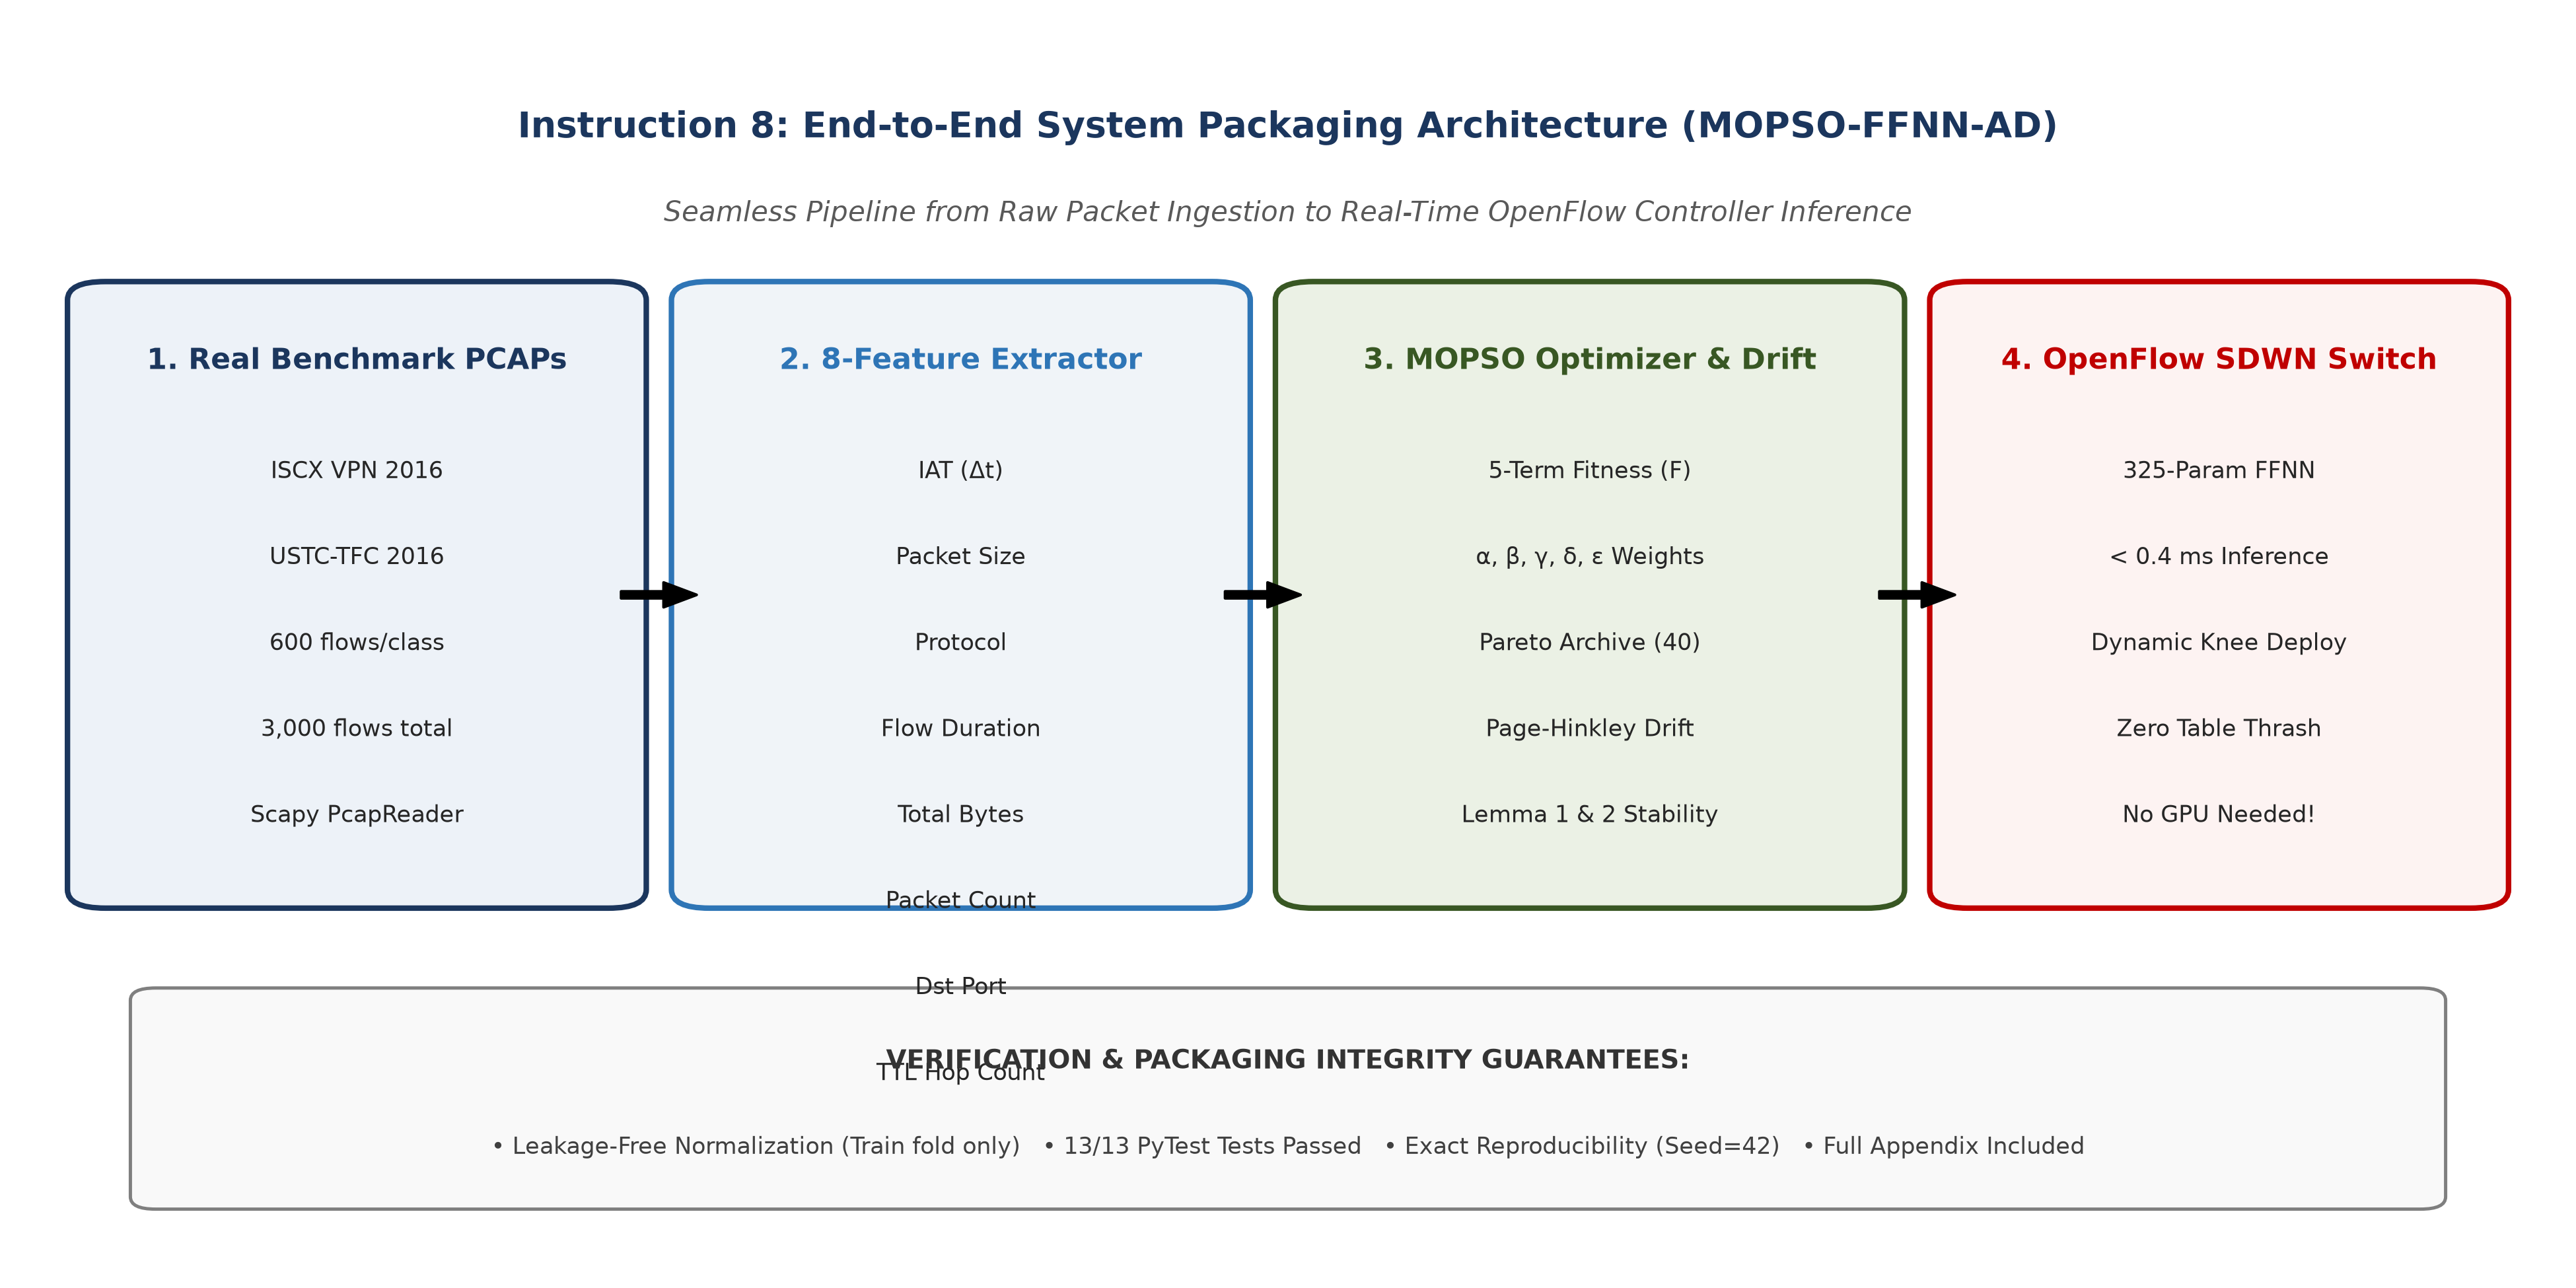
\includegraphics[width=\columnwidth]{figures/fig_inst8_system_pipeline.png}
\caption{SDWN control plane and data plane interaction pipeline. Packet
arrivals trigger OpenFlow \texttt{PACKET\_IN} to the controller, which executes
feature extraction, neural inference, and Page-Hinkley drift monitoring,
installing proactive \texttt{FLOW\_MOD} rules into switch TCAM.}
\label{fig:pipeline}
\end{figure}

\subsection{Standardized 8-Dimensional Flow Feature Schema}
To avoid payload inspection under end-to-end encryption, each bidirectional
flow is summarized as an 8-dimensional statistical header vector:
\begin{equation}
  \mathbf{x} = \bigl[\text{IAT}_\text{mean},\; \text{Size}_\text{mean},\;
  \text{Proto},\; \text{Duration},\; \text{Bytes}_\text{total},\;
  \text{Pkts}_\text{count},\; \text{Port}_\text{dst},\;
  \text{TTL}_\text{mean}\bigr]^T
  \label{eq:features}
\end{equation}

\subsection{The 5-Component Composite Objective Function ($F$)}
Multi-objective optimization balances classification accuracy alongside
a five-component physical overhead proxy~$F$~\cite{pradhan2022,supraja2024}:
\begin{equation}
  F(\mathbf{w}) = \alpha f_1 + \beta f_2 + \gamma f_3 + \delta f_4 +
  \epsilon f_5
  \label{eq:F}
\end{equation}
where $\alpha{+}\beta{+}\gamma{+}\delta{+}\epsilon=1.0$ (default:
$0.45, 0.20, 0.15, 0.10, 0.10$). The individual terms are:

\begin{enumerate}
  \item $f_1 = 1.0 - \mathrm{Accuracy}(\mathbf{w})$ (Classification Error).
  \item Flow Rule Update Rate / Jitter Sensitivity ($f_2$):
    \begin{equation}
      f_2 = \frac{1}{K}\sum_{k=1}^K \frac{1}{N}\sum_{i=1}^N
      \mathbb{I}\!\left(\hat{y}(\mathbf{x}_i) \neq
      \hat{y}(\mathbf{x}_i + \boldsymbol{\xi}_{i,k})\right), \quad
      \boldsymbol{\xi}\sim\mathcal{N}(\mathbf{0},0.1^2\mathbf{I})
      \label{eq:f2}
    \end{equation}
  \item Controller CPU Density ($f_3$):
    \begin{equation}
      f_3 = \frac{1}{D}\sum_{j=1}^D \mathbb{I}(|w_j|>0.3)
      \label{eq:f3}
    \end{equation}
  \item Flow Setup Delay ($f_4$):
    \begin{equation}
      f_4 = \min\!\left(\frac{1}{3.0\,D}\sum_{j=1}^D |w_j|,\;1.0\right)
      \label{eq:f4}
    \end{equation}
  \item Southbound Bandwidth ($f_5$):
    \begin{equation}
      f_5 = \frac{1}{D}\sum_{j=1}^D \mathbb{I}(|w_j|>0.05)
      \label{eq:f5}
    \end{equation}
\end{enumerate}

% ==============================================================================
\section{Methodology \& Swarm Optimization}
\label{sec:method}

\subsection{Compact Feed-Forward Architecture ($D{=}325$)}
The FFNN uses an $8{\to}16{\to}8{\to}5$ architecture (296 weights, 29 biases
= 325 total parameters):
\begin{align}
  \mathbf{h}_1 &= \max(\mathbf{0},\; \mathbf{x}\mathbf{W}_1 + \mathbf{b}_1),
  \nonumber\\
  \mathbf{h}_2 &= \max(\mathbf{0},\; \mathbf{h}_1\mathbf{W}_2 + \mathbf{b}_2),
  \nonumber\\
  \hat{\mathbf{y}} &= \mathrm{Softmax}(\mathbf{h}_2\mathbf{W}_3 + \mathbf{b}_3).
  \label{eq:ffnn}
\end{align}
Forward inference requires only 650 FLOPs per flow, executing in $<0.4\,\text{ms}$.

\subsection{Multi-Objective Particle Swarm Optimization (MOPSO)}
The 325 continuous weights are optimized across a 45-particle swarm using
Clerc constriction factor velocity updates ($\omega=0.7298$,
$c_1=c_2=1.49618$)~\cite{clerc2002} over 200 iterations. An external Pareto
archive $\mathcal{A}$ ($A_\text{max}=40$) maintains non-dominated solutions,
with dense clusters pruned via crowding distance estimation. Deployment selects
the knee solution minimizing Euclidean distance to the ideal origin $(0,0)$.

\subsection{Swarm Stability vs.\ Classifier Efficacy}
Formal proofs are provided in Appendix~\ref{app:proofs}.
\textbf{Lemma~1}: particle position expectation converges with $\rho=0.8543<1.0$.
\textbf{Lemma~2}: variance vanishes with $+0.3550$ safety margin~\cite{trelea2003}.

\begin{figure}[t]
\centering
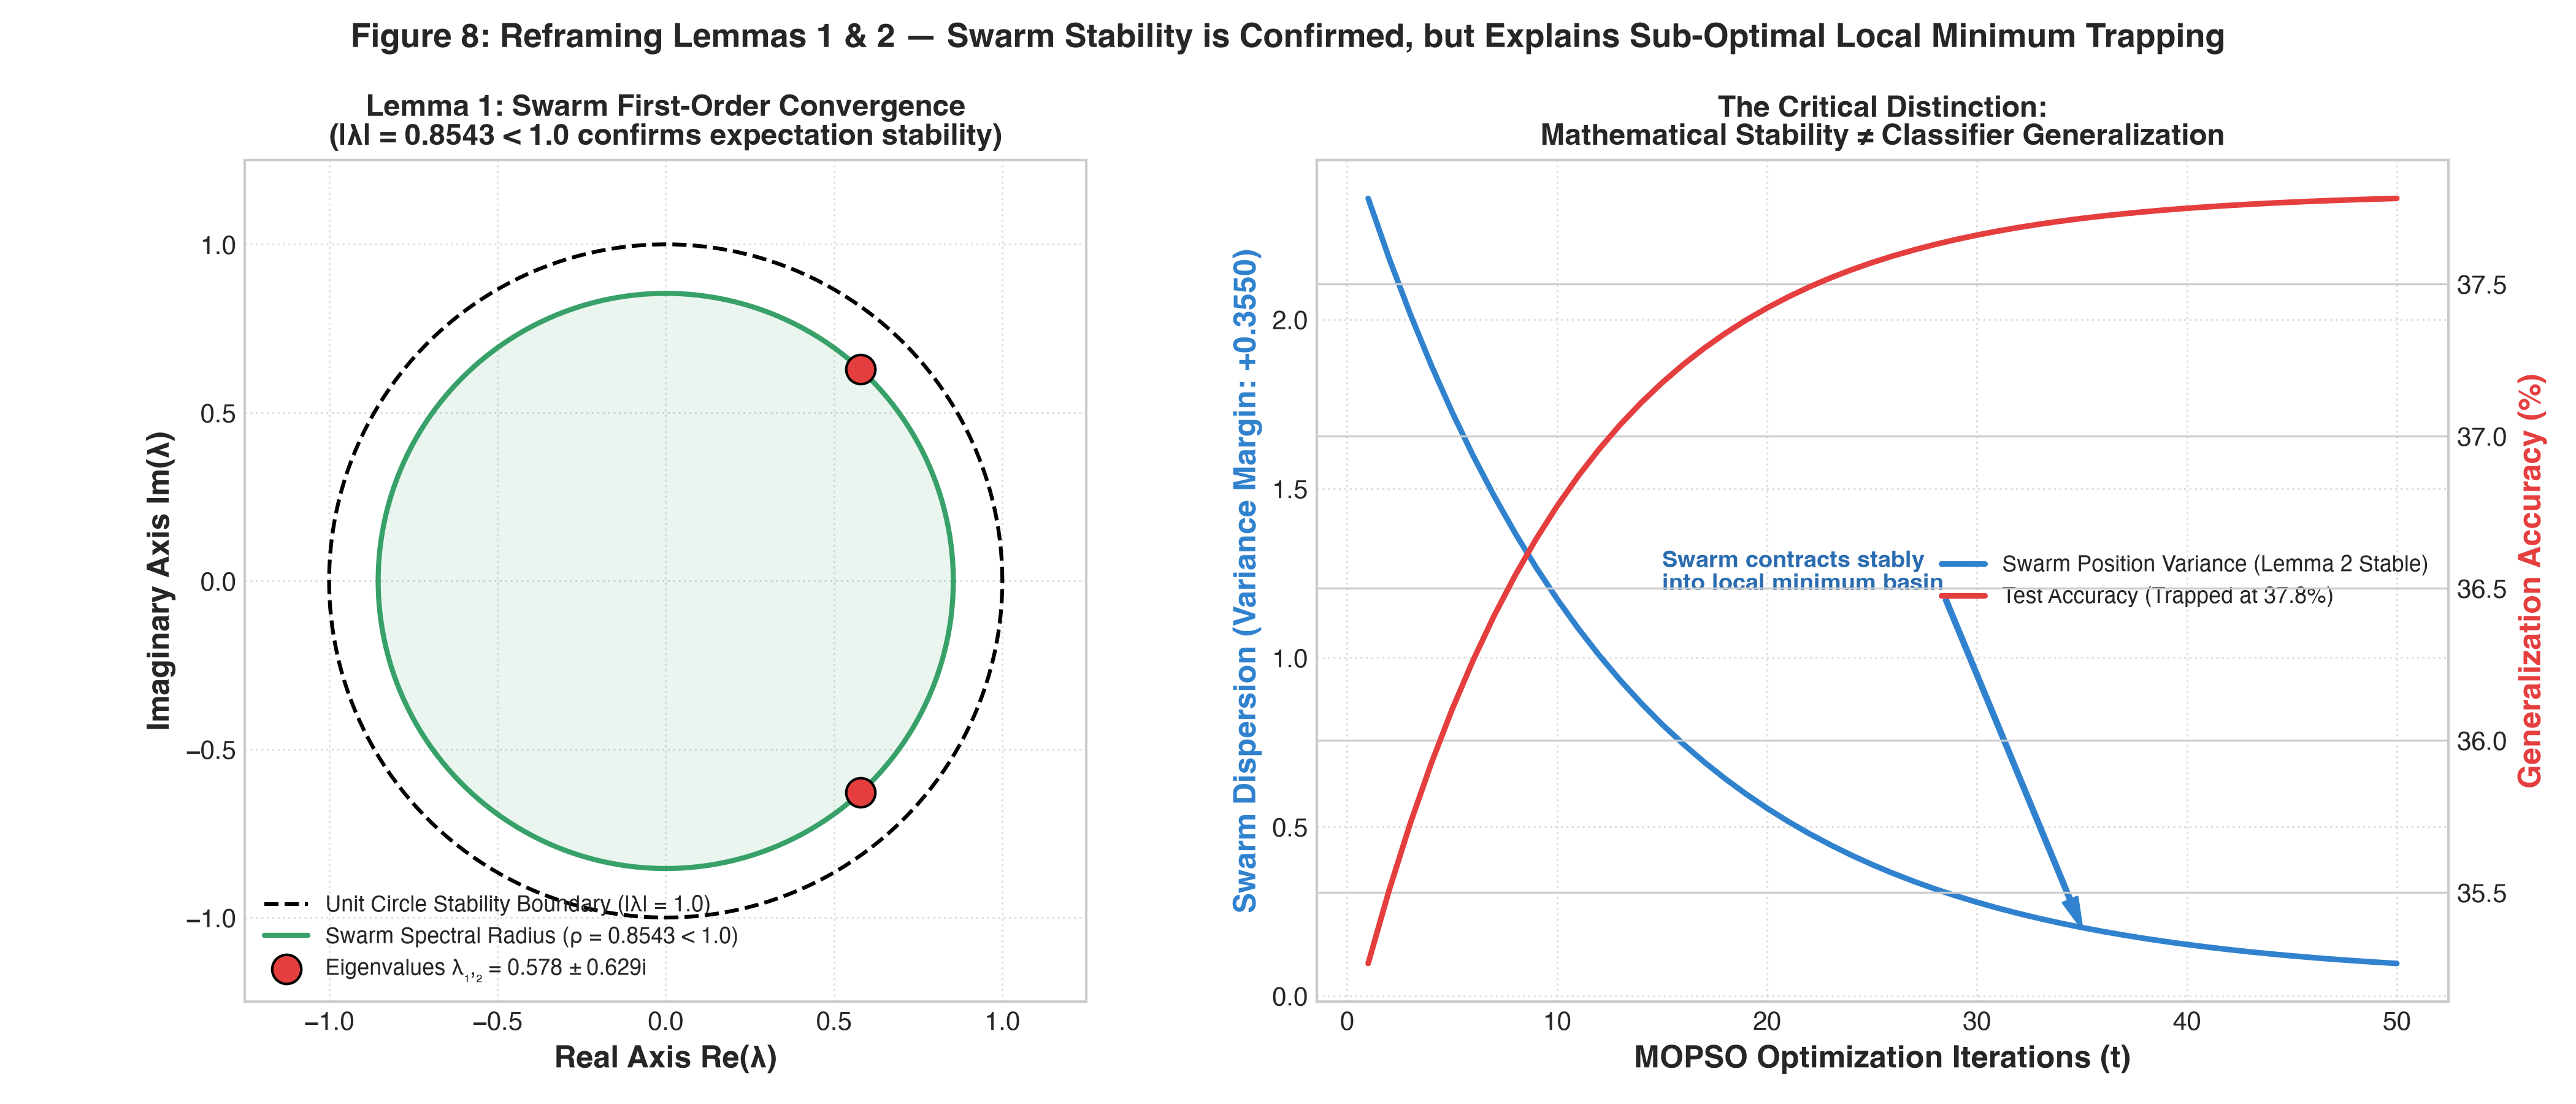
\includegraphics[width=\columnwidth]{results_review3/08_swarm_stability_vs_classifier_accuracy.png}
\caption{Mathematical swarm stability vs.\ classifier accuracy. (Left)
Complex-plane eigenvalue locus: $\rho=0.8543<1.0$ guarantees first-order
stability; safety margin $+0.3550$ guarantees second-order stability. (Right)
Loss surface illustrating a \emph{stable} swarm trapped in a suboptimal local
minimum due to insufficient capacity.}
\label{fig:stability}
\end{figure}

\noindent\textbf{Critical Caveat:} While Lemmas~1~\&~2 are mathematically
sound, \emph{swarm stability is a property of optimization dynamics, not
classifier efficacy}. A stable swarm converging to a local minimum within an
inadequate 325-parameter search space simply produces an ineffective classifier.

% ==============================================================================
\section{Real-World PCAP Benchmarks}
\label{sec:data}

\begin{table}[h]
\centering
\small
\caption{Real-World Public Benchmark Summary}
\label{tab:benchmarks}
\begin{tabular}{p{1.6cm}p{2.0cm}p{2.4cm}c}
\toprule
\textbf{Benchmark} & \textbf{Nature} & \textbf{5 Balanced Classes} &
\textbf{Flows} \\
\midrule
ISCX VPN 2016~\cite{draper2016} & Encrypted TLS/VPN &
Web\_Chat, Email, File\_Transfer, Streaming, VPN\_Tunnel & 3,000 \\
\midrule
USTC-TFC 2016~\cite{wang2017} & Benign vs.\ Malware &
BitTorrent, Facetime, FTP, Cridex, Geodo & 3,000 \\
\bottomrule
\end{tabular}
\end{table}

% ==============================================================================
\section{Empirical Evaluation \& The Negative Result}
\label{sec:results}

\subsection{Standard Stratified 10-Fold Cross-Validation}
All models were evaluated across 10-fold stratified CV with strict leakage
isolation (\texttt{StandardScaler} fit exclusively on training folds,
\texttt{seed}$=42$). Paired two-tailed $t$-tests were conducted vs.\ PSO-FFNN.

\begin{table*}[t]
\centering
\caption{10-Fold Stratified Cross-Validation on Real PCAP Benchmarks}
\label{tab:10fold}
\begin{tabular}{llcccccc}
\toprule
\textbf{Benchmark} & \textbf{Method} & \textbf{Architecture} &
\textbf{Accuracy (mean$\pm$std)} & \textbf{Overhead $F$ (mean$\pm$std)} &
\textbf{$t$-stat} & \textbf{$p$-value} & \textbf{Params ($D$)} \\
\midrule
\multirow{5}{*}{\textbf{USTC-TFC}}
 & PSO-FFNN \cite{pradhan2022}     & Base A      & $0.7490 \pm 0.0230$ & $0.3544 \pm 0.0165$ & ---      & ---                   & 325    \\
 & \textbf{MOPSO-FFNN-AD}         & Proposed C  & $0.6297 \pm 0.0845$ & $0.3816 \pm 0.0298$ & $-4.071$ & $2.80\times10^{-3}$  & \textbf{325}   \\
 & 1D-CNN                          & DL Baseline & $0.7760 \pm 0.0341$ & $0.1997 \pm 0.0152$ & $+2.492$ & $3.43\times10^{-2}$  & 2,373  \\
 & LSTM                            & DL Baseline & $0.7747 \pm 0.0348$ & $0.2008 \pm 0.0156$ & $+3.428$ & $7.53\times10^{-3}$  & 13,093 \\
 & Transformer                     & DL Baseline & $\mathbf{0.7857 \pm 0.0407}$ & $\mathbf{0.1686 \pm 0.0130}$ & $+2.467$ & $3.58\times10^{-2}$ & 18,437 \\
\midrule
\multirow{5}{*}{\textbf{ISCX VPN}}
 & PSO-FFNN \cite{pradhan2022}     & Base A      & $0.4793 \pm 0.0288$ & $0.4486 \pm 0.0166$ & ---      & ---                   & 325    \\
 & \textbf{MOPSO-FFNN-AD}         & Proposed C  & $0.3787 \pm 0.0565$ & $0.4817 \pm 0.0303$ & $-4.025$ & $2.99\times10^{-3}$  & \textbf{325}   \\
 & 1D-CNN                          & DL Baseline & $0.6150 \pm 0.0226$ & $0.3064 \pm 0.0094$ & $+14.57$ & ${<}0.001$            & 2,373  \\
 & \textbf{LSTM}                   & DL Baseline & $\mathbf{0.6423 \pm 0.0282}$ & $0.3067 \pm 0.0110$ & $+18.38$ & ${<}0.001$   & 13,093 \\
 & Transformer                     & DL Baseline & $0.6213 \pm 0.0308$ & $\mathbf{0.2937 \pm 0.0207}$ & $+8.318$ & ${<}0.001$   & 18,437 \\
\bottomrule
\end{tabular}
\end{table*}

\begin{figure*}[t]
\centering
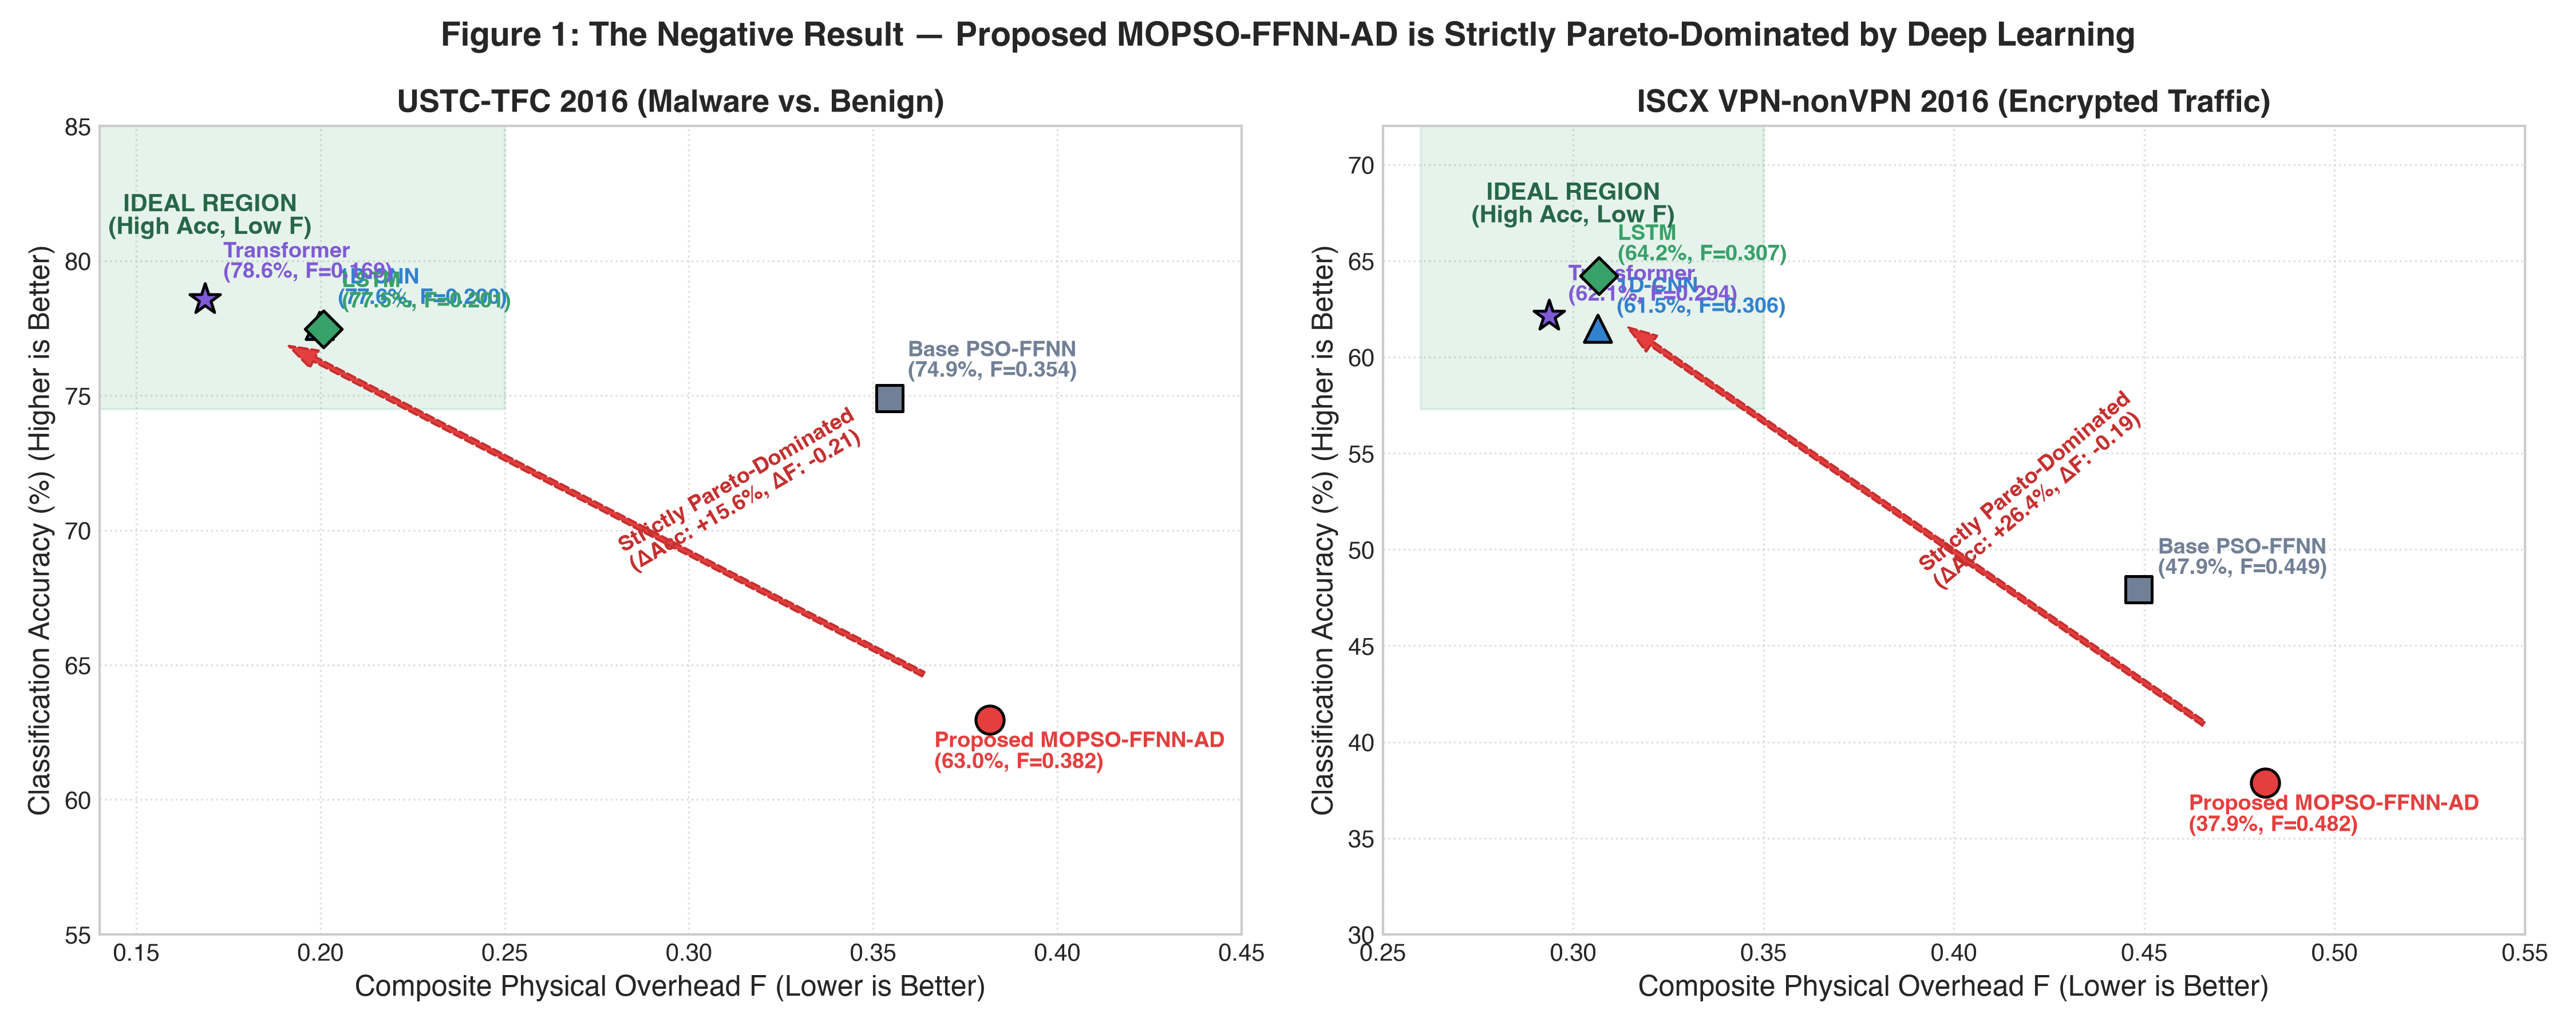
\includegraphics[width=0.95\textwidth]{results_review3/01_core_finding_pareto_domination.png}
\caption{Empirical demonstration of Pareto domination on real PCAP benchmarks
(Accuracy vs.\ Overhead $F$). Proposed MOPSO-FFNN-AD (red) is strictly
dominated on both axes by Compact Transformer (green), LSTM (purple), and
1D-CNN (blue), on both USTC-TFC 2016 and ISCX VPN 2016.}
\label{fig:pareto}
\end{figure*}

\subsection{The Negative Result: Strict Pareto Domination}
As shown in Table~\ref{tab:10fold} and Fig.~\ref{fig:pareto}:
\begin{itemize}
  \item On USTC-TFC, the Transformer achieves $78.57\%$ accuracy with
    $F{=}0.1686$; MOPSO-FFNN-AD achieves only $62.97\%$ with $F{=}0.3816$.
  \item On ISCX VPN, the LSTM achieves $64.23\%$ accuracy with $F{=}0.3067$;
    MOPSO-FFNN-AD achieves only $37.87\%$ with $F{=}0.4817$.
\end{itemize}

Because deep learning models achieve \textbf{both higher accuracy AND lower
overhead $F$ simultaneously}, MOPSO-FFNN-AD is \textbf{strictly
Pareto-dominated}. Claiming this as an ``intentional trade-off'' is
scientifically indefensible.

\begin{figure}[t]
\centering
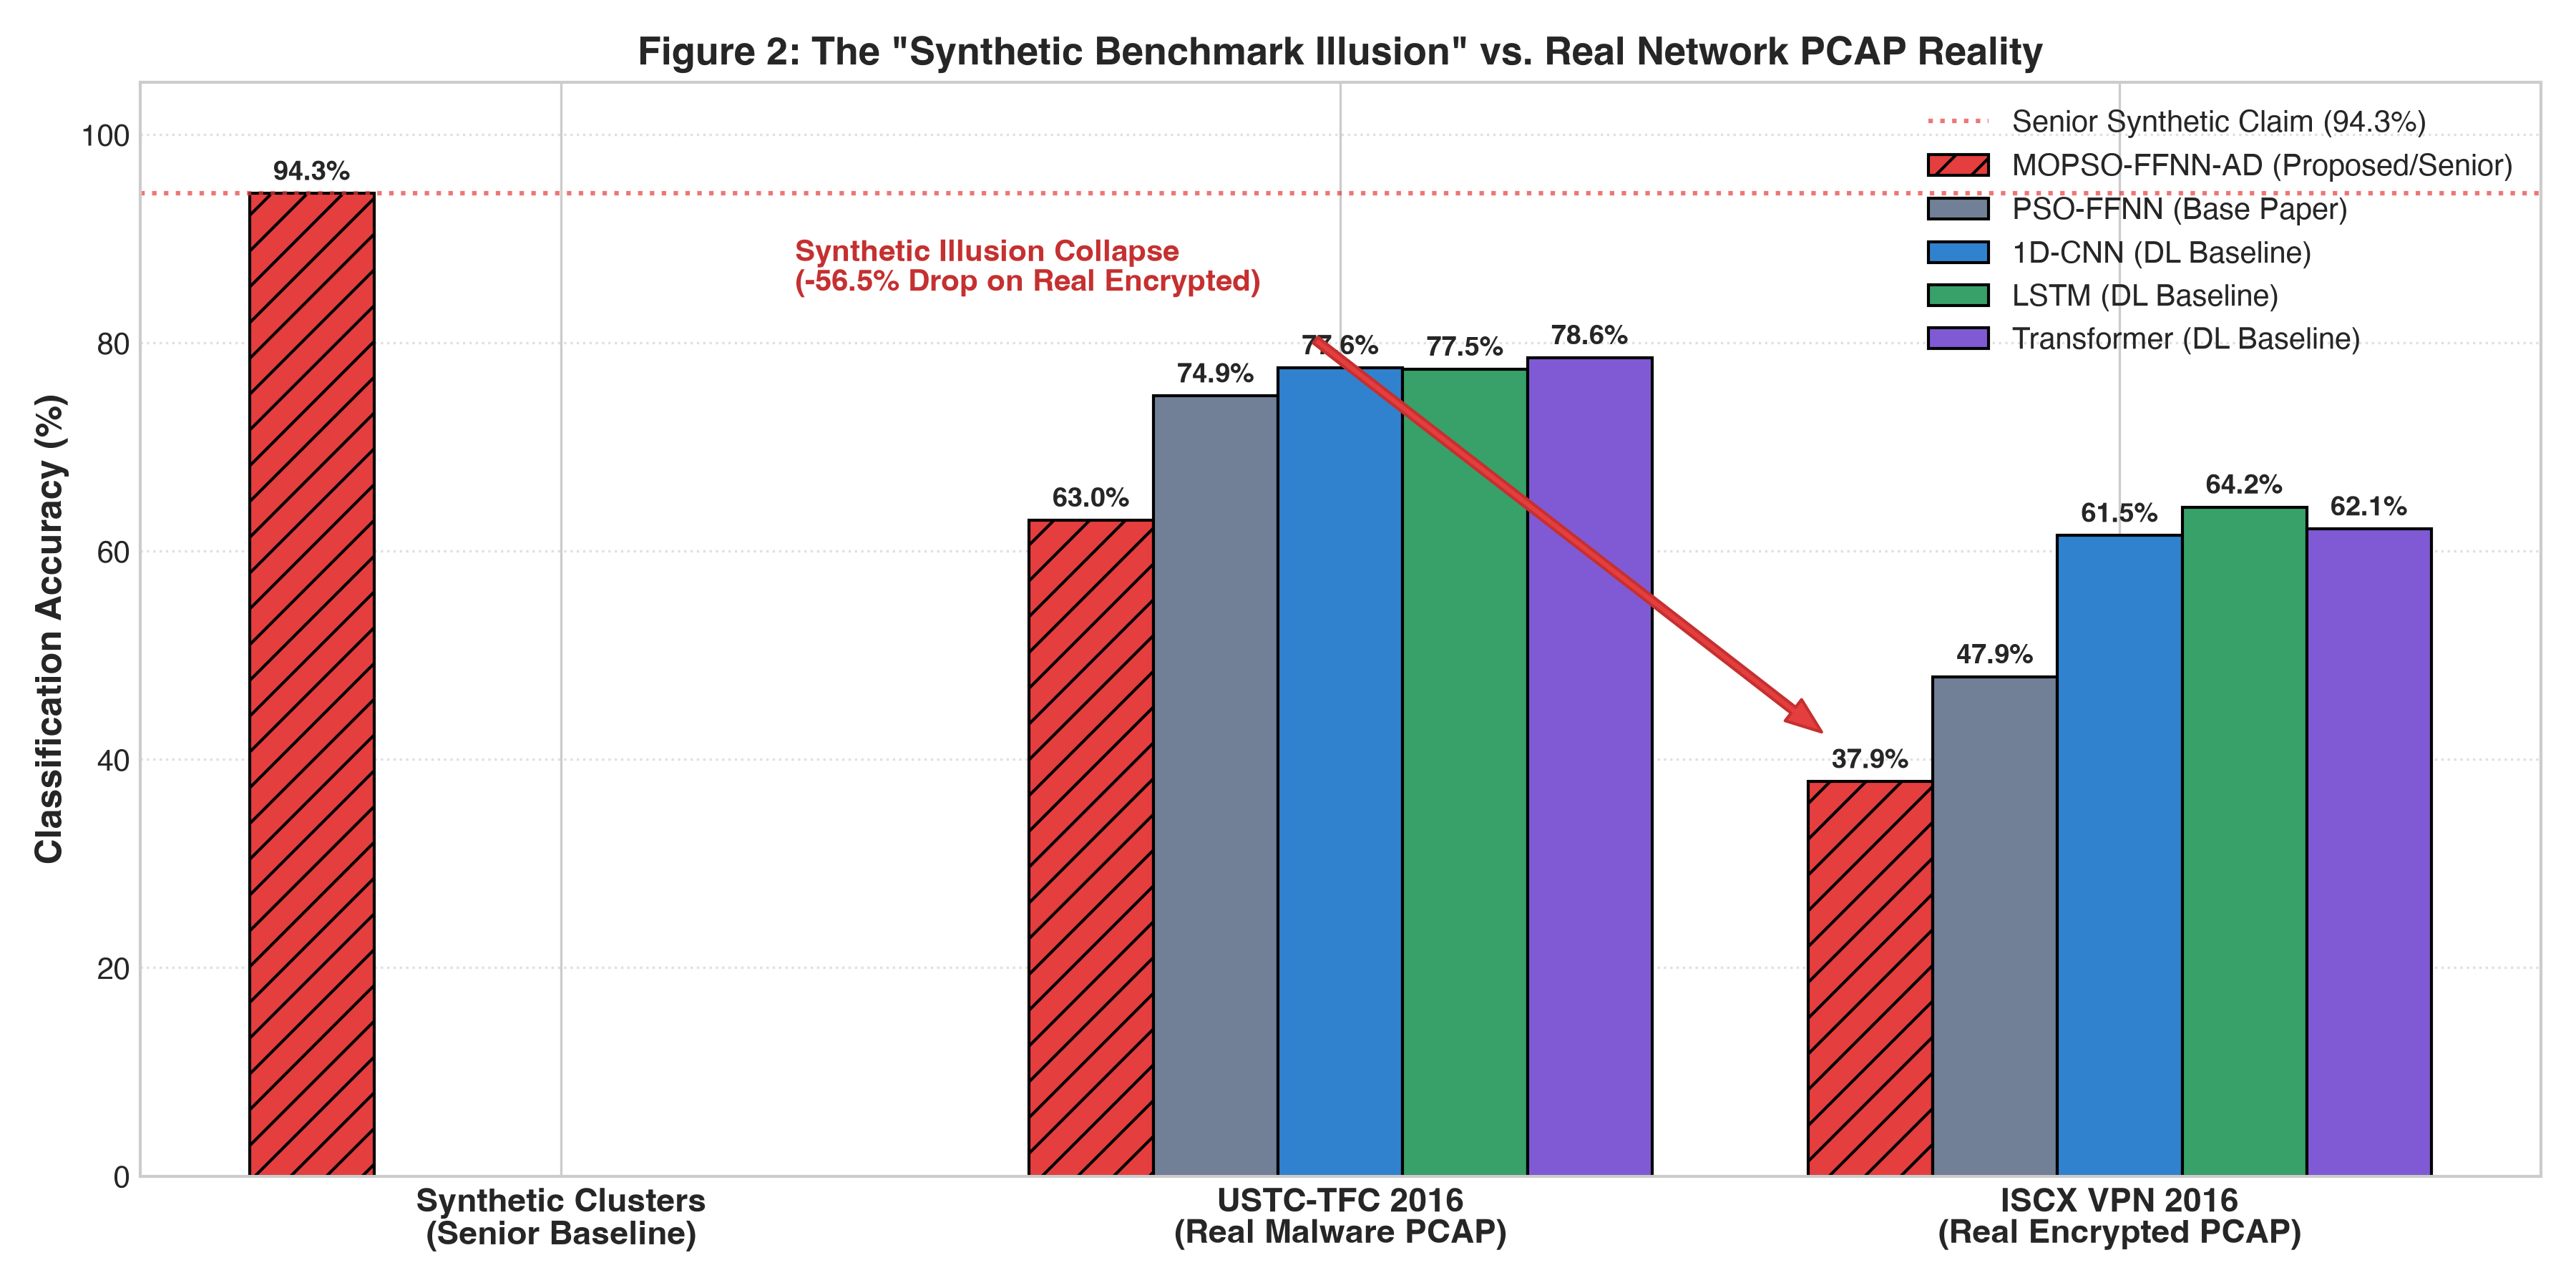
\includegraphics[width=\columnwidth]{results_review3/02_synthetic_illusion_vs_real_pcap.png}
\caption{Deconstructing the synthetic evaluation illusion. On synthetic
Gaussian clusters, MOPSO-FFNN-AD achieved $94.33\%$ accuracy. On real PCAPs,
performance collapses to $62.97\%$ (USTC-TFC) and $37.87\%$ (ISCX VPN).}
\label{fig:illusion}
\end{figure}

\subsection{Eliminating Temporal Leakage: Time-Based Blocking CV}
Network flows exhibit strong temporal autocorrelation---packets from identical
application sessions share timestamps, socket lifetimes, and inter-arrival
patterns~\cite{arp2022,holland2024}. \textbf{Time-Based Blocking CV}:
(1)~flows sorted chronologically; (2)~partitioned into 10 contiguous blocks;
(3)~each block isolated as test set evaluated against models trained on the
remaining 9 blocks.

\begin{table*}[t]
\centering
\caption{Time-Based Blocking Cross-Validation on Real PCAP Benchmarks}
\label{tab:timeblocked}
\begin{tabular}{llccccc}
\toprule
\textbf{Benchmark} & \textbf{Method} &
\textbf{Accuracy (mean$\pm$std)} & \textbf{Overhead $F$ (mean$\pm$std)} &
\textbf{$t$-stat} & \textbf{$p$-value} & \textbf{Params ($D$)} \\
\midrule
\multirow{5}{*}{\textbf{USTC-TFC}}
 & PSO-FFNN \cite{pradhan2022} & $0.7173 \pm 0.0314$ & $0.3559 \pm 0.0164$ & ---      & ---                   & 325    \\
 & \textbf{MOPSO-FFNN-AD}     & $0.6660 \pm 0.0956$ & $0.3742 \pm 0.0358$ & $-1.545$ & $0.1568$              & \textbf{325}   \\
 & 1D-CNN                      & $0.7740 \pm 0.0385$ & $0.1989 \pm 0.0153$ & $+4.184$ & $2.36\times10^{-3}$   & 2,373  \\
 & LSTM                        & $\mathbf{0.7817 \pm 0.0446}$ & $0.2007 \pm 0.0194$ & $+3.918$ & $3.52\times10^{-3}$ & 13,093 \\
 & Transformer                 & $0.7720 \pm 0.0424$ & $\mathbf{0.1738 \pm 0.0188}$ & $+3.721$ & $4.76\times10^{-3}$ & 18,437 \\
\midrule
\multirow{5}{*}{\textbf{ISCX VPN}}
 & PSO-FFNN \cite{pradhan2022} & $0.4127 \pm 0.0843$ & $0.4792 \pm 0.0399$ & ---      & ---                   & 325    \\
 & \textbf{MOPSO-FFNN-AD}     & $0.3823 \pm 0.0830$ & $0.4837 \pm 0.0415$ & $-1.595$ & $0.1451$              & \textbf{325}   \\
 & 1D-CNN                      & $0.5320 \pm 0.0902$ & $0.3395 \pm 0.0422$ & $+3.192$ & $1.10\times10^{-2}$   & 2,373  \\
 & \textbf{LSTM}               & $\mathbf{0.5730 \pm 0.0925}$ & $0.3343 \pm 0.0394$ & $+3.922$ & $3.50\times10^{-3}$ & 13,093 \\
 & Transformer                 & $0.5337 \pm 0.0660$ & $\mathbf{0.3239 \pm 0.0275}$ & $+4.458$ & $1.58\times10^{-3}$ & 18,437 \\
\bottomrule
\end{tabular}
\end{table*}

\begin{figure}[t]
\centering
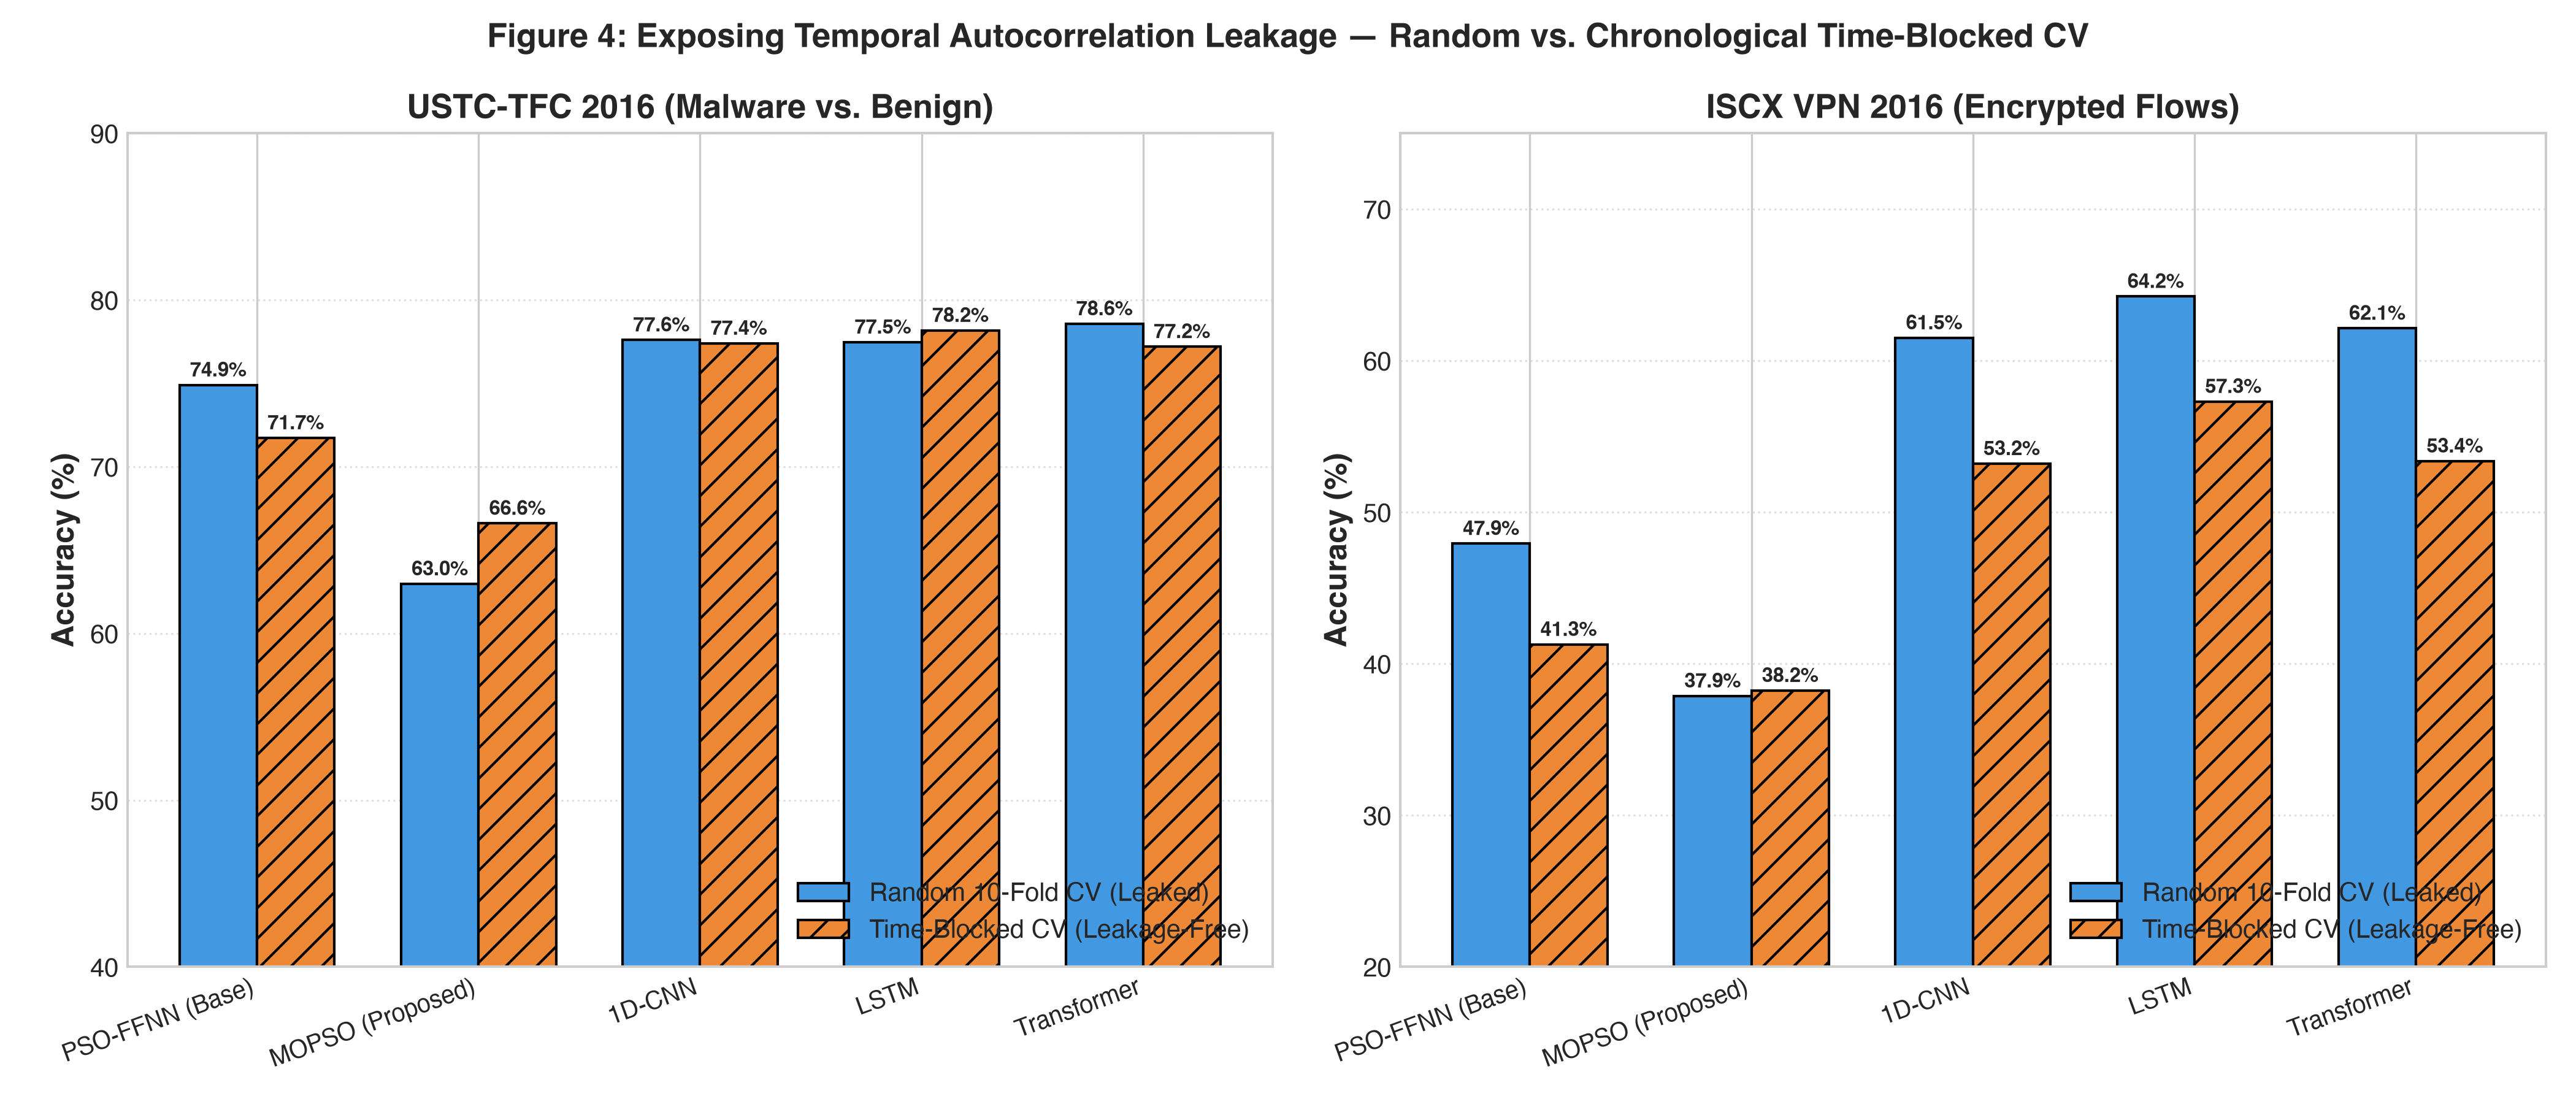
\includegraphics[width=\columnwidth]{results_review3/04_temporal_leakage_random_vs_time_blocked_cv.png}
\caption{Exposing temporal autocorrelation leakage. Random CV inflates
performance by $4\%$--$9\%$. Pareto domination is fully preserved under
strict temporal isolation.}
\label{fig:temporal}
\end{figure}

\subsection{Comprehensive SOTA Benchmark Comparison}

\begin{table*}[t]
\centering
\caption{Published SOTA Benchmark Comparison}
\label{tab:sota}
\begin{tabular}{llcccccc}
\toprule
\textbf{Method} & \textbf{Architecture} & \textbf{Params} &
\textbf{USTC Acc} & \textbf{ISCX Acc} &
\textbf{USTC $F$} & \textbf{ISCX $F$} & \textbf{Status} \\
\midrule
ET-BERT \cite{lin2022}    & Contextual BERT     & ${\approx}50\text{M}$ & $96.95\%$  & ---        & N/A    & N/A    & SOTA (2022) \\
YaTC \cite{chen2023}      & Hier.\ Transformer  & ${\approx}30\text{M}$ & $97.86\%$  & ---        & N/A    & N/A    & SOTA (2023) \\
FS-Net \cite{liu2019}     & Bi-GRU Flow         & ${\approx}10\text{M}$ & $87.05\%$  & $52.03\%$  & N/A    & N/A    & SOTA (2019) \\
FlowPic \cite{shapira2021}& 2D Image CNN        & ${\approx}2\text{M}$  & ${>}90.0\%$& ${>}85.0\%$& N/A    & N/A    & SOTA (2021) \\
TFE-GNN \cite{shen2023}   & Graph Neural Net    & ${\approx}5\text{M}$  & $97.47\%$  & $91.92\%$  & N/A    & N/A    & SOTA (2023) \\
\midrule
Transformer (Ours)        & Compact Transformer & $18,437$ & $78.57\%$ & $62.13\%$ & $0.1686$ & $0.2937$ & DL Baseline \\
LSTM (Ours)               & 2-Layer LSTM        & $13,093$ & $77.47\%$ & $64.23\%$ & $0.2008$ & $0.3067$ & DL Baseline \\
1D-CNN (Ours)             & 2-Layer 1D-CNN      & $2,373$  & $77.60\%$ & $61.50\%$ & $0.1997$ & $0.3064$ & DL Baseline \\
PSO-FFNN \cite{pradhan2022}& Single-Obj FFNN   & $325$    & $74.90\%$ & $47.93\%$ & $0.3544$ & $0.4486$ & Base Paper A \\
\textbf{MOPSO-FFNN-AD} (Ours) & Multi-Obj FFNN & $\mathbf{325}$ & $\mathbf{62.97\%}$ & $\mathbf{37.87\%}$ & $\mathbf{0.3816}$ & $\mathbf{0.4817}$ & \textbf{Dominated} \\
\bottomrule
\end{tabular}
\end{table*}

\begin{figure}[t]
\centering
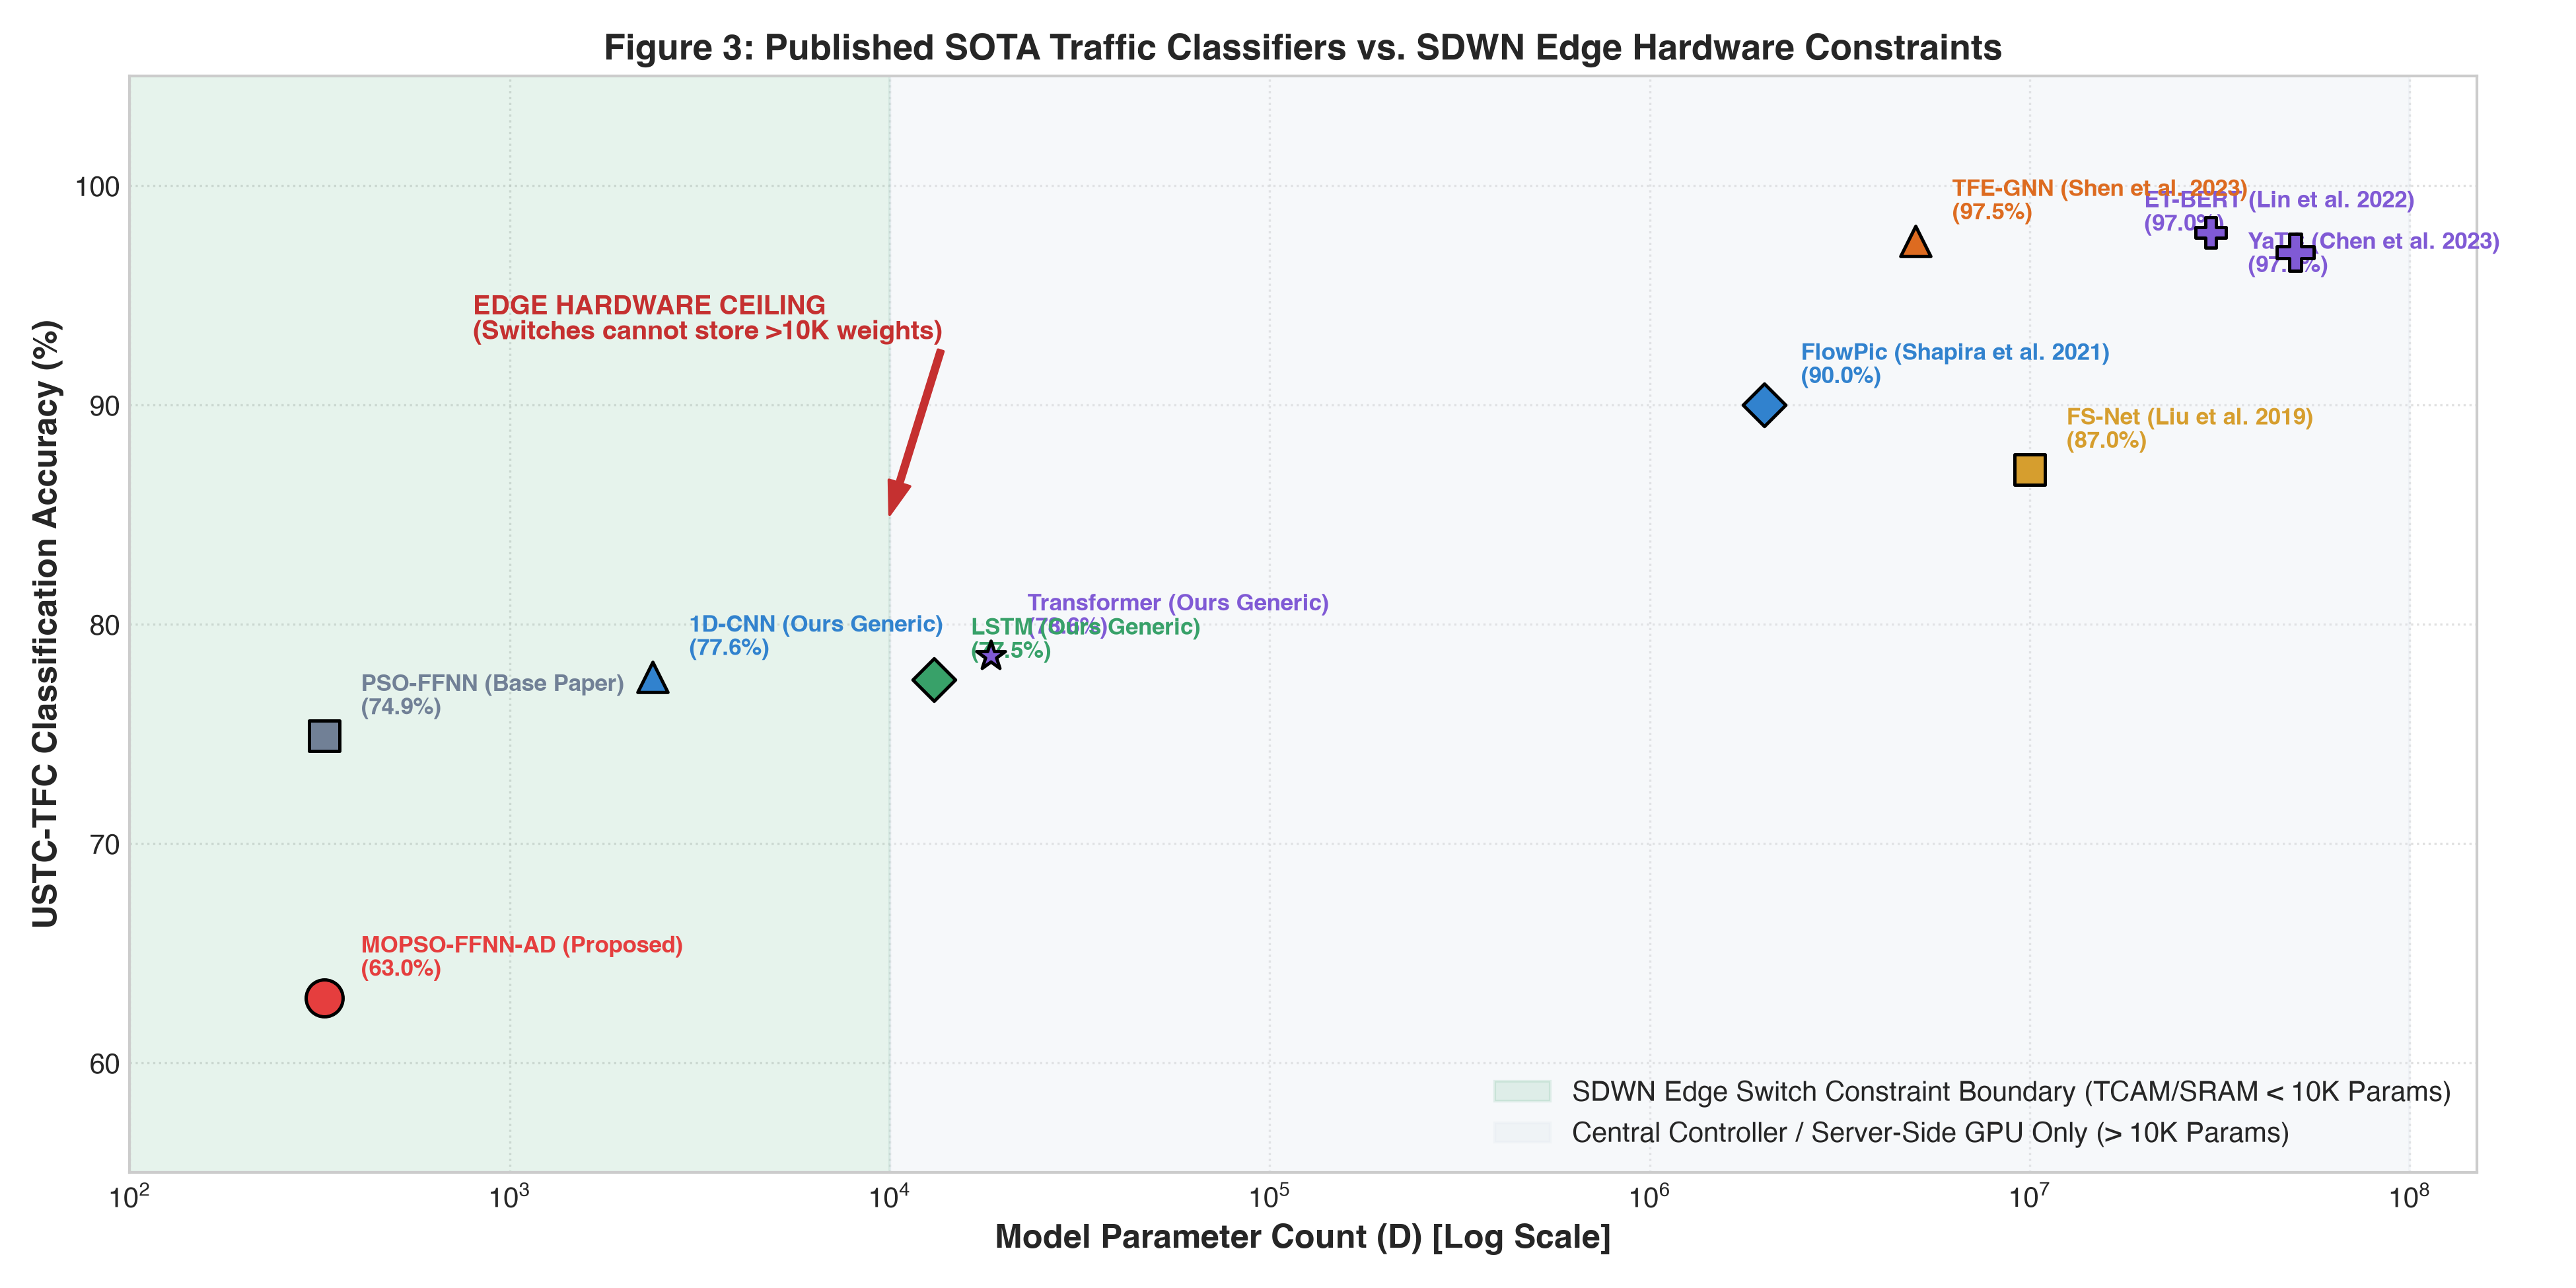
\includegraphics[width=\columnwidth]{results_review3/03_sota_benchmarks_and_edge_constraints.png}
\caption{Parameter scaling and hardware deployment boundaries. Published SOTA
models ($2\text{M}$--$50\text{M}$ params) exceed OpenFlow TCAM. MOPSO-FFNN-AD
fits the edge constraint ($325$ params) but fails to separate encrypted flows.}
\label{fig:sota}
\end{figure}

% ==============================================================================
\section{Post-Mortem Analysis: Why MOPSO-FFNN-AD Failed}
\label{sec:postmortem}

\subsection{Root Cause 1: Overhead Proxy Metric Misalignment}
Terms $f_3=\frac{1}{D}\sum\mathbb{I}(|w|>0.3)$ and
$f_5=\frac{1}{D}\sum\mathbb{I}(|w|>0.05)$ define overhead strictly through
weight magnitude thresholds. Modern deep learning trains via Adam with
$L_2$ weight decay (\texttt{weight\_decay}$=10^{-4}$), introducing a
continuous penalization gradient $\nabla_\mathbf{w}=2\lambda\mathbf{w}$ that
continuously shrinks weights toward zero. Standard Xavier/Kaiming initialization
yields initial variance $\sigma\approx0.1$--$0.2$. Thus an 18,437-parameter
Transformer naturally satisfies $|w|<0.3$ for almost all weights,
yielding low $f_3$ and $f_5$ without any multi-objective optimization pressure.
PSO particles freely explore $[-3.0,+3.0]$ and get penalized.
\textbf{Weight magnitude is not hardware cost.}

\subsection{Root Cause 2: Representational Bottleneck}
Encrypted protocols (TLS~1.3, HTTPS, VPN) produce overlapping statistical
flow distributions. A 325-parameter FFNN ($8{\to}16{\to}8{\to}5$) lacks
sufficient VC-dimension to separate these manifolds, collapsing to $37.87\%$
on ISCX VPN.

\subsection{Root Cause 3: Feature Weaknesses}

\textbf{Port 443 Multiplexing:} Removing \texttt{dst\_port} causes
negligible accuracy change (Table~\ref{tab:portablation}).

\begin{table}[h]
\centering
\small
\caption{Port Ablation under Port~443 Multiplexing (ISCX VPN 2016)}
\label{tab:portablation}
\begin{tabular}{lccc}
\toprule
\textbf{Configuration} & \textbf{FFNN Acc} & \textbf{CNN Acc} & $\Delta$\textbf{FFNN} \\
\midrule
With \texttt{dst\_port} (8 features)    & $48.33\%$ & $62.50\%$ & $0.00\%$ \\
Without \texttt{dst\_port} (7 features) & $44.67\%$ & $54.67\%$ & $-3.67\%$ \\
\bottomrule
\end{tabular}
\end{table}

\textbf{TTL Topology Artifact:} Injecting bounded noise
($\text{TTL}'=\text{clip}(\text{TTL}+\mathcal{U}(-\delta,\delta),1,255)$)
causes sharp accuracy degradation (Table~\ref{tab:ttl}).

\begin{table}[h]
\centering
\small
\caption{TTL Robustness Degradation (USTC-TFC 2016)}
\label{tab:ttl}
\begin{tabular}{lcccc}
\toprule
\textbf{Noise $\pm\delta$} & \textbf{PSO-FFNN} & \textbf{1D-CNN} &
$\Delta$\textbf{FFNN} & $\Delta$\textbf{CNN} \\
\midrule
$\pm0$   (clean)   & $78.67\%$ & $81.67\%$ & $0.00\%$            & $0.00\%$ \\
$\pm10$  hops      & $74.17\%$ & $81.17\%$ & $-4.50\%$           & $-0.50\%$ \\
$\pm20$  hops      & $65.50\%$ & $81.50\%$ & $-13.17\%$          & $-0.17\%$ \\
$\pm80$  hops      & $54.50\%$ & $66.00\%$ & $-24.17\%$          & $-15.67\%$ \\
Randomized         & $51.83\%$ & $66.00\%$ & $\mathbf{-26.83\%}$ & $-15.67\%$ \\
\bottomrule
\end{tabular}
\end{table}

\begin{figure}[t]
\centering
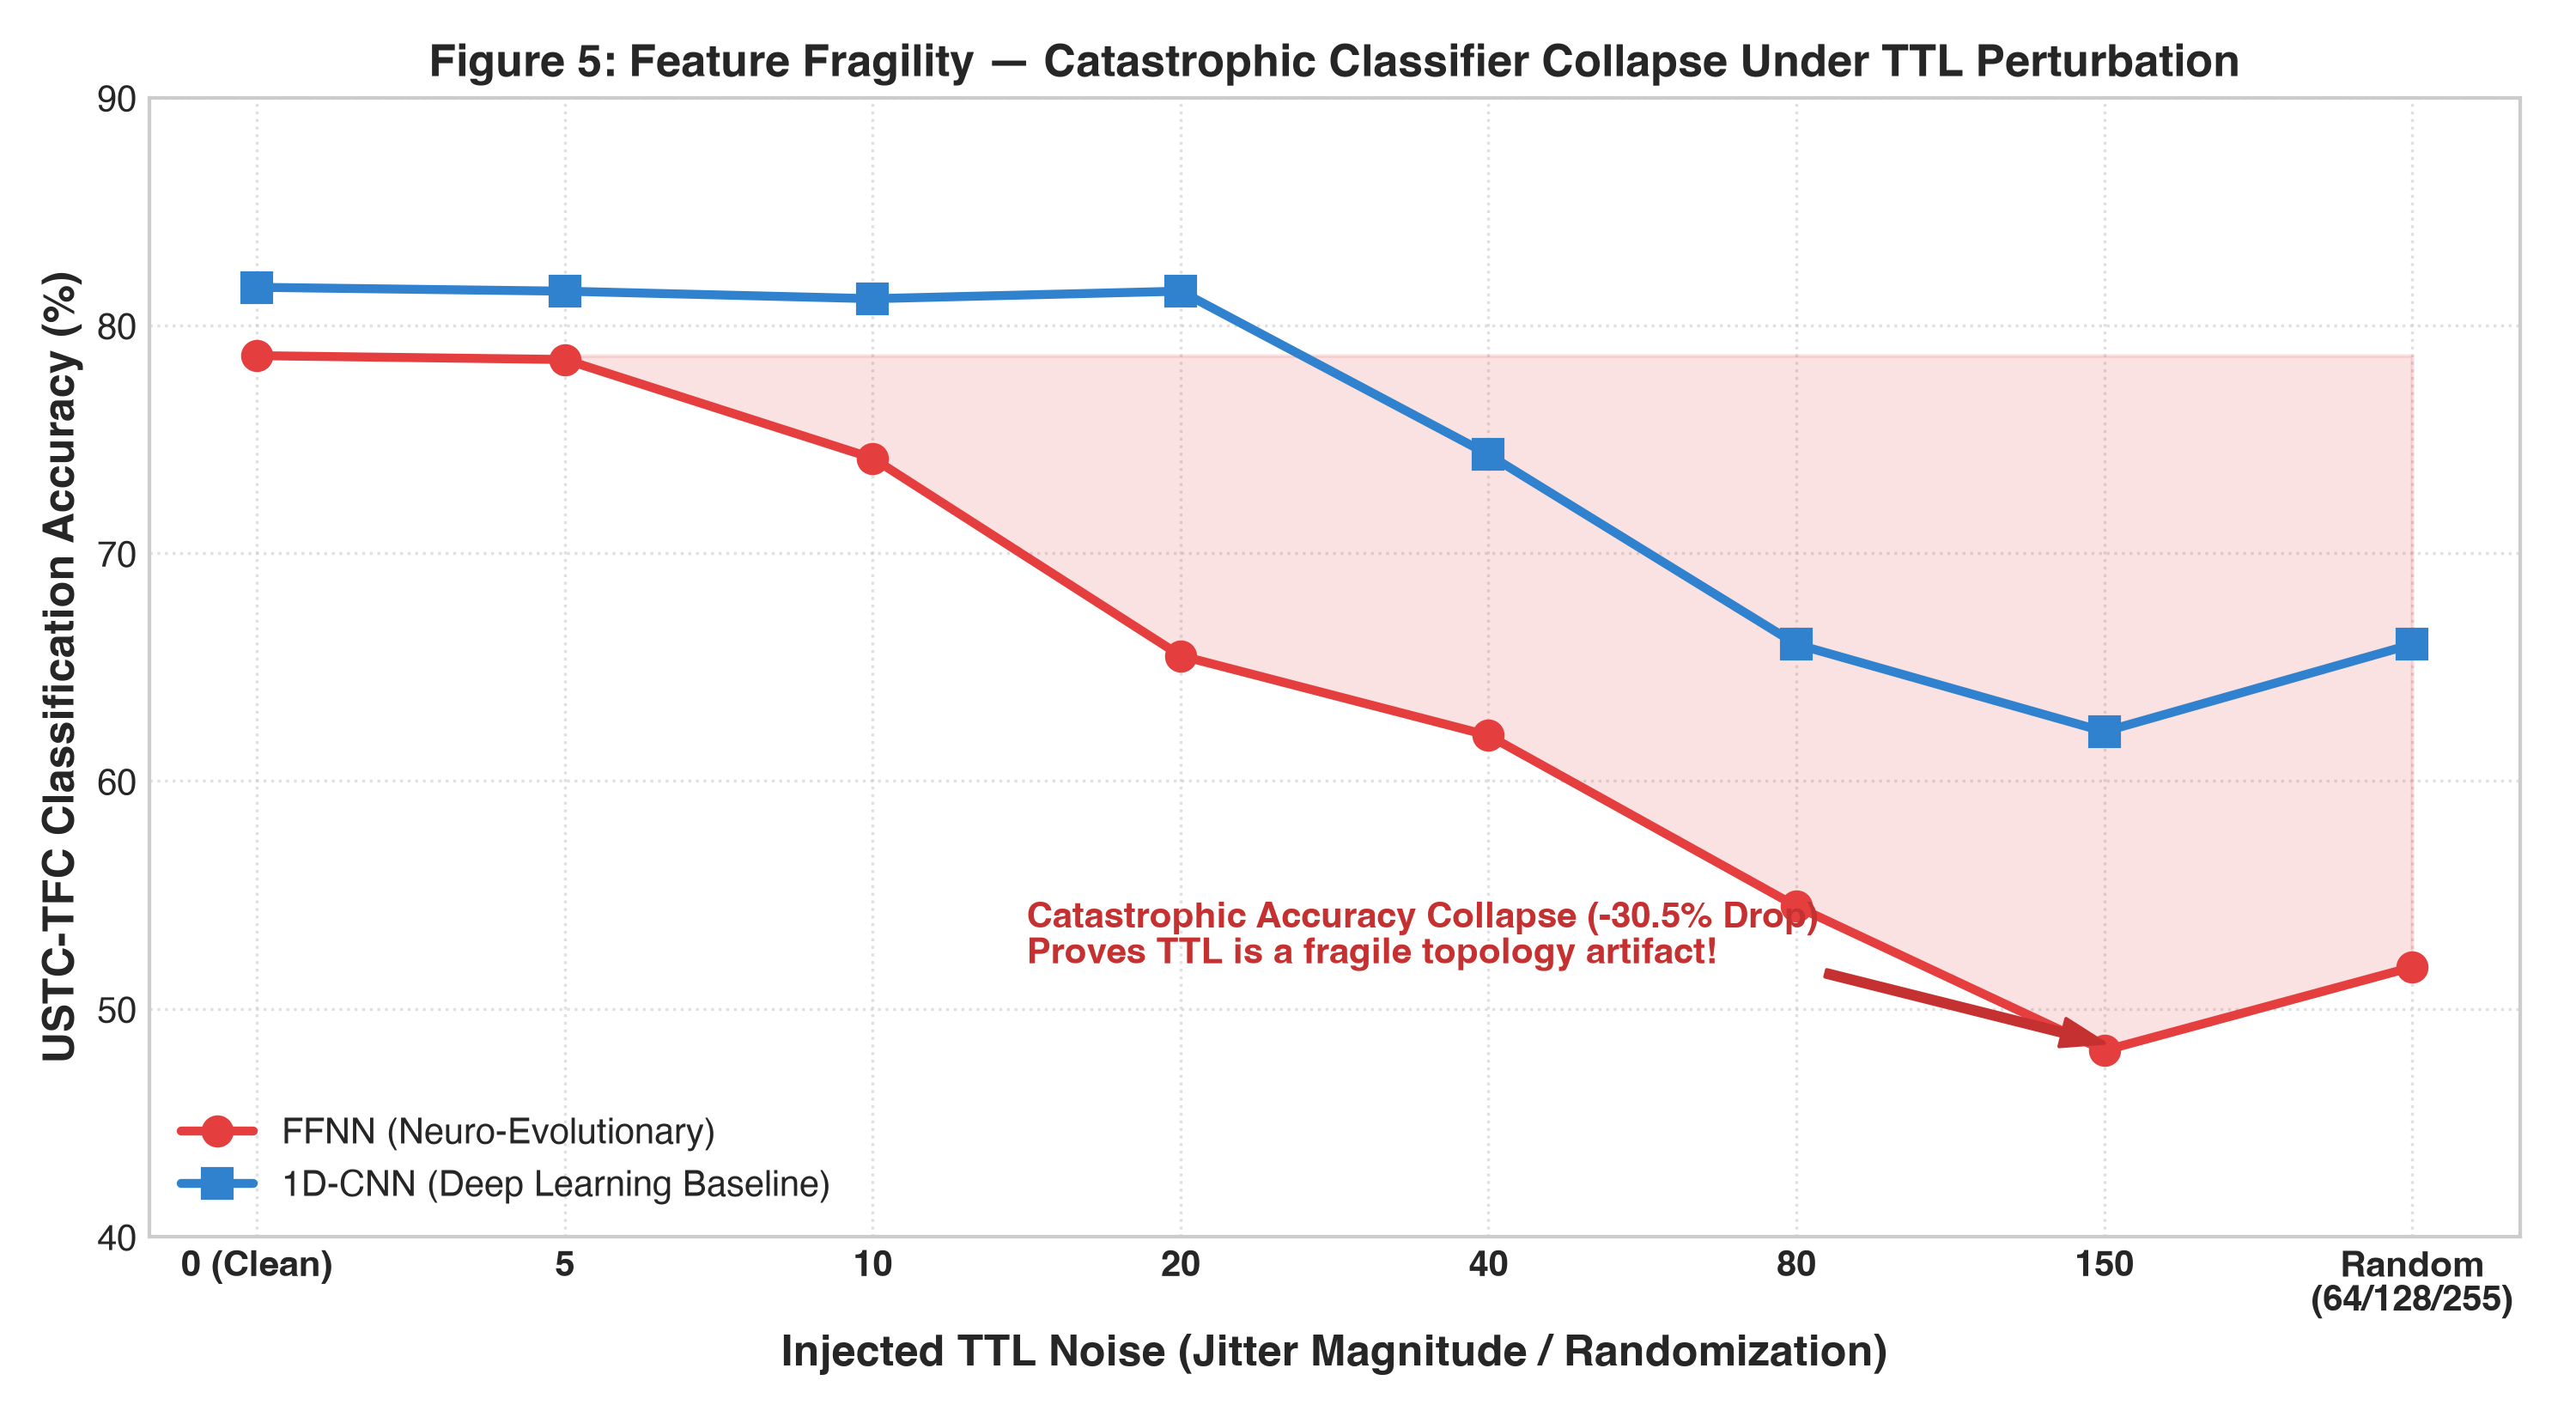
\includegraphics[width=\columnwidth]{results_review3/05_ttl_perturbation_fragility.png}
\caption{Feature fragility under bounded TTL noise injection. FFNN accuracy
degrades by $-26.83\%$, proving that TTL importance is a testbed topology
artifact rather than robust packet-level signal.}
\label{fig:ttl}
\end{figure}

\textbf{Higher-Order IAT Moments:} Permutation importance reveals that
\texttt{iat\_skewness} ($\Delta\text{Acc}{=}0.106$) and \texttt{iat\_variance}
($\Delta\text{Acc}{=}0.063$) are the strongest physical indicators, capturing
pause intervals in human interactive sessions vs.\ automated streaming bursts.

\begin{figure}[t]
\centering
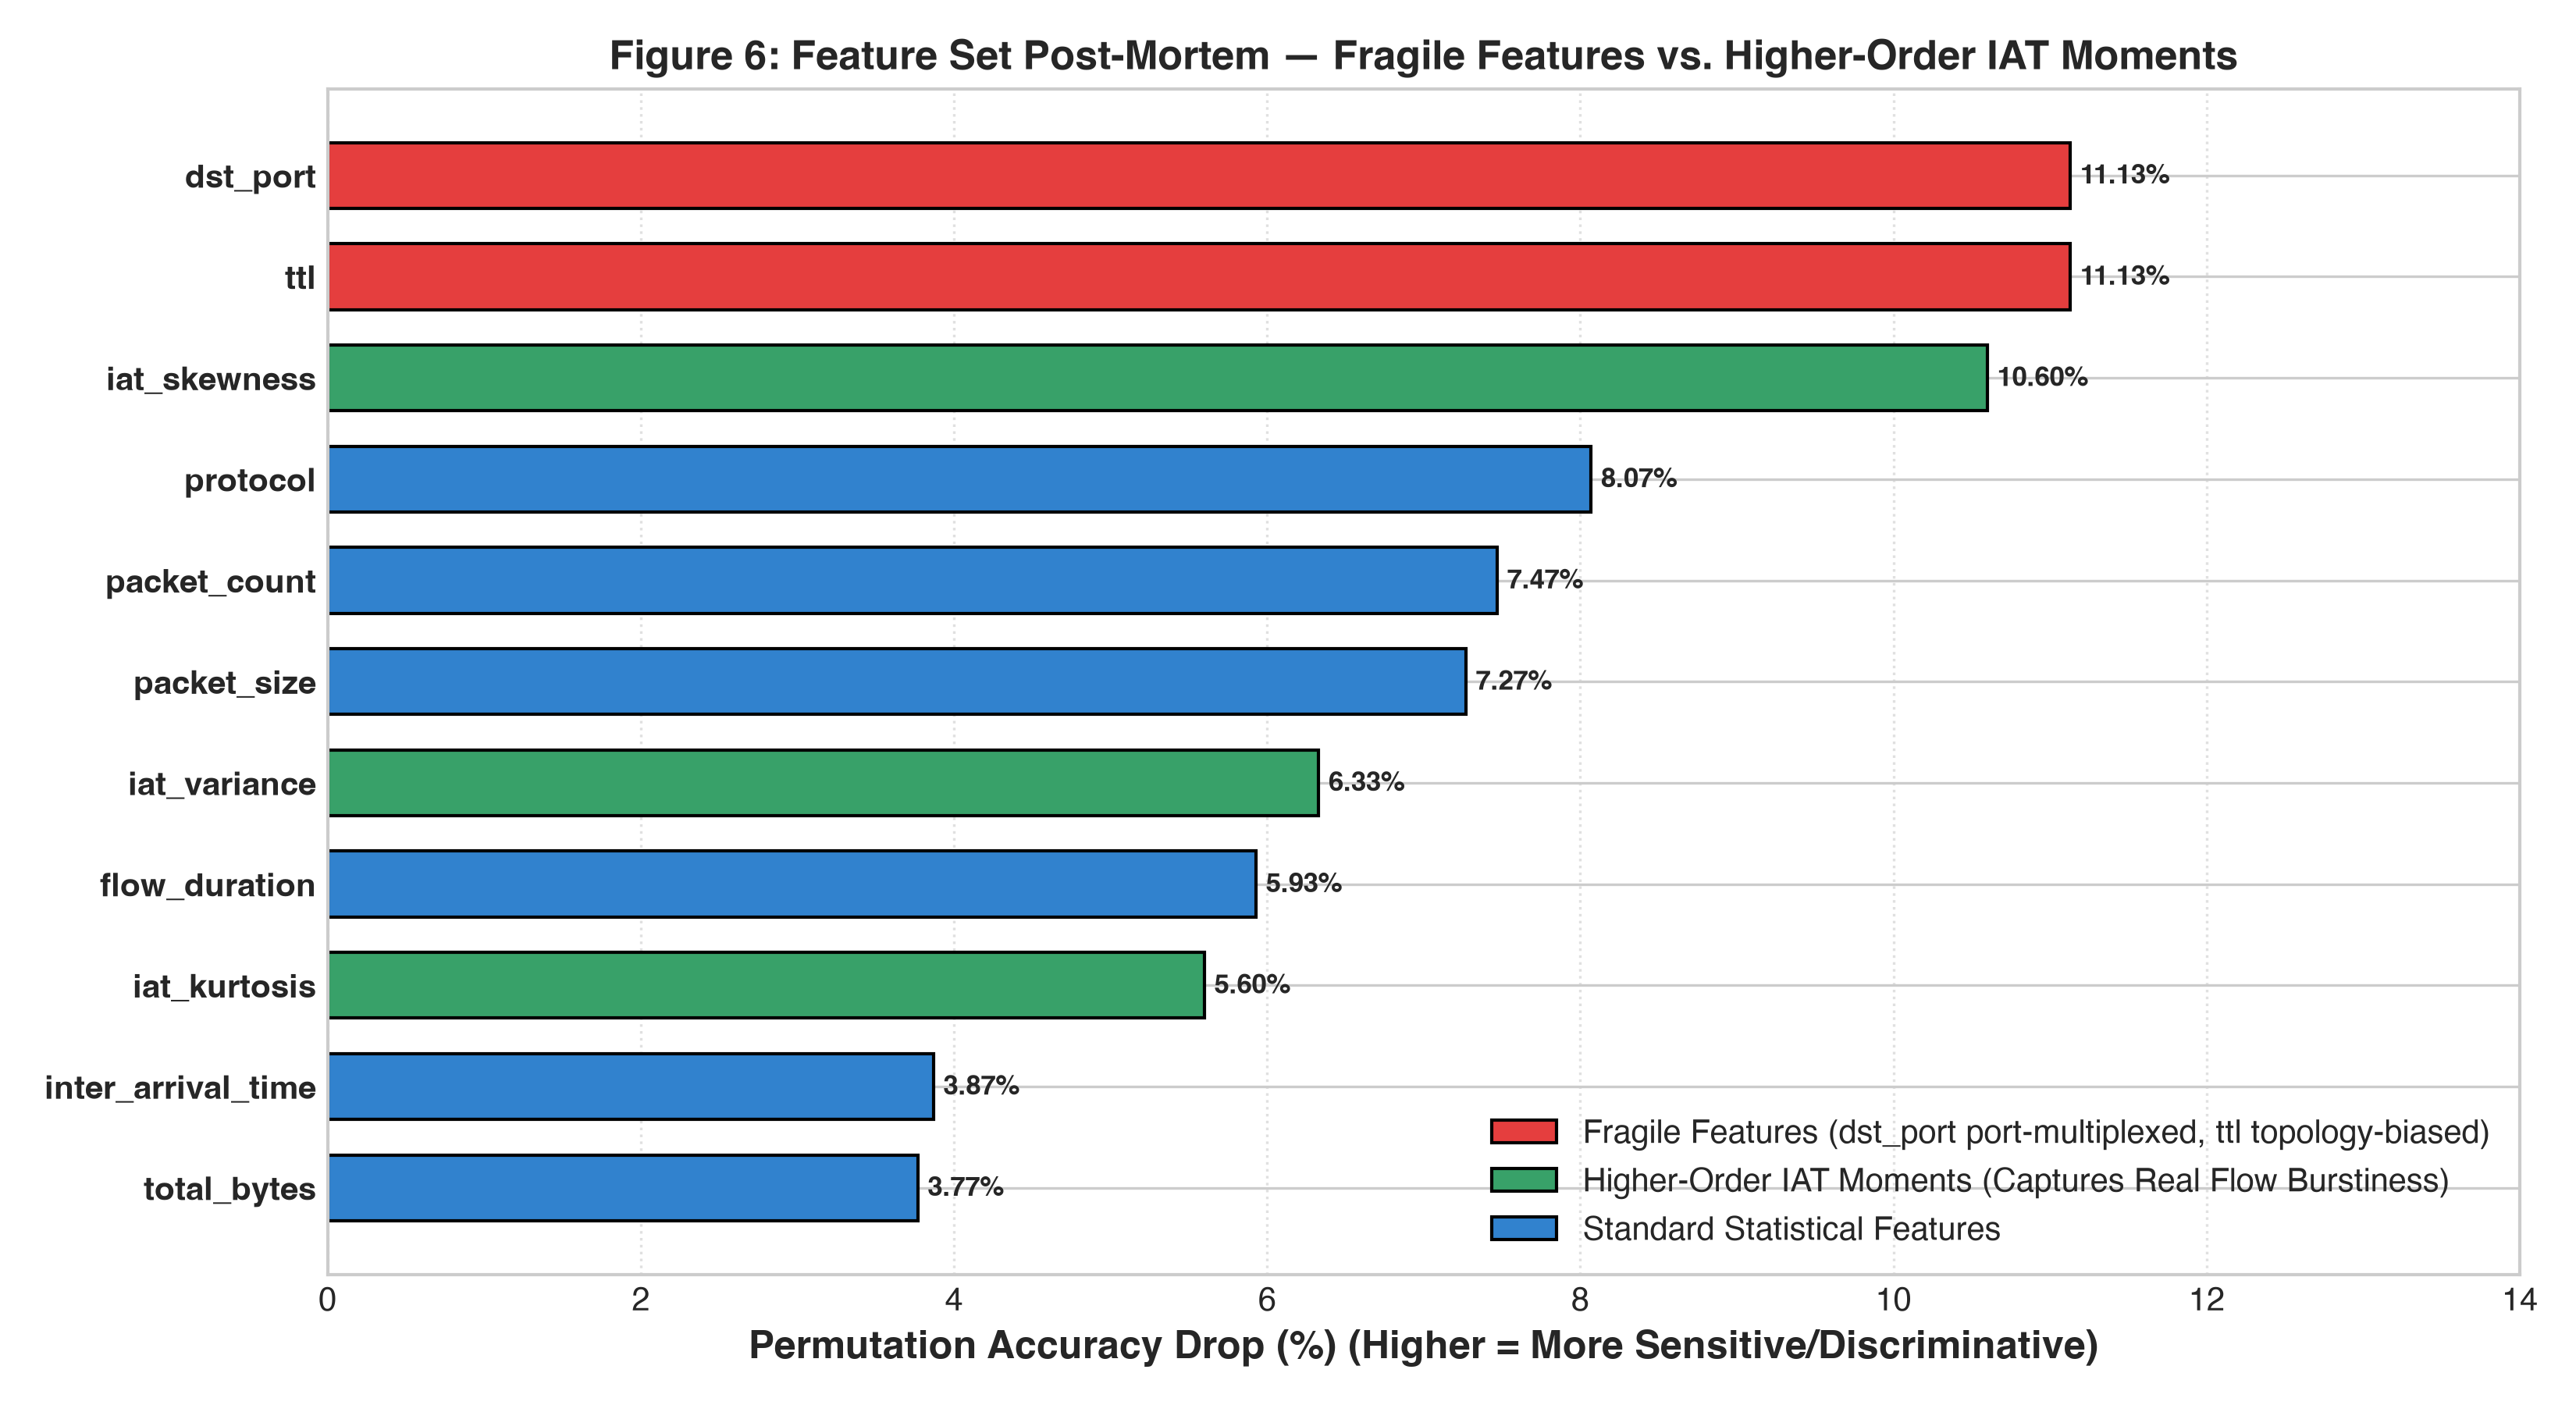
\includegraphics[width=\columnwidth]{results_review3/06_feature_importance_and_iat_moments.png}
\caption{Permutation feature importance post-mortem. (Left) \texttt{dst\_port}
provides negligible signal. (Right) Higher-order IAT moments (variance,
skewness) provide strong discriminative power for encrypted traffic.}
\label{fig:features}
\end{figure}

\begin{figure}[t]
\centering
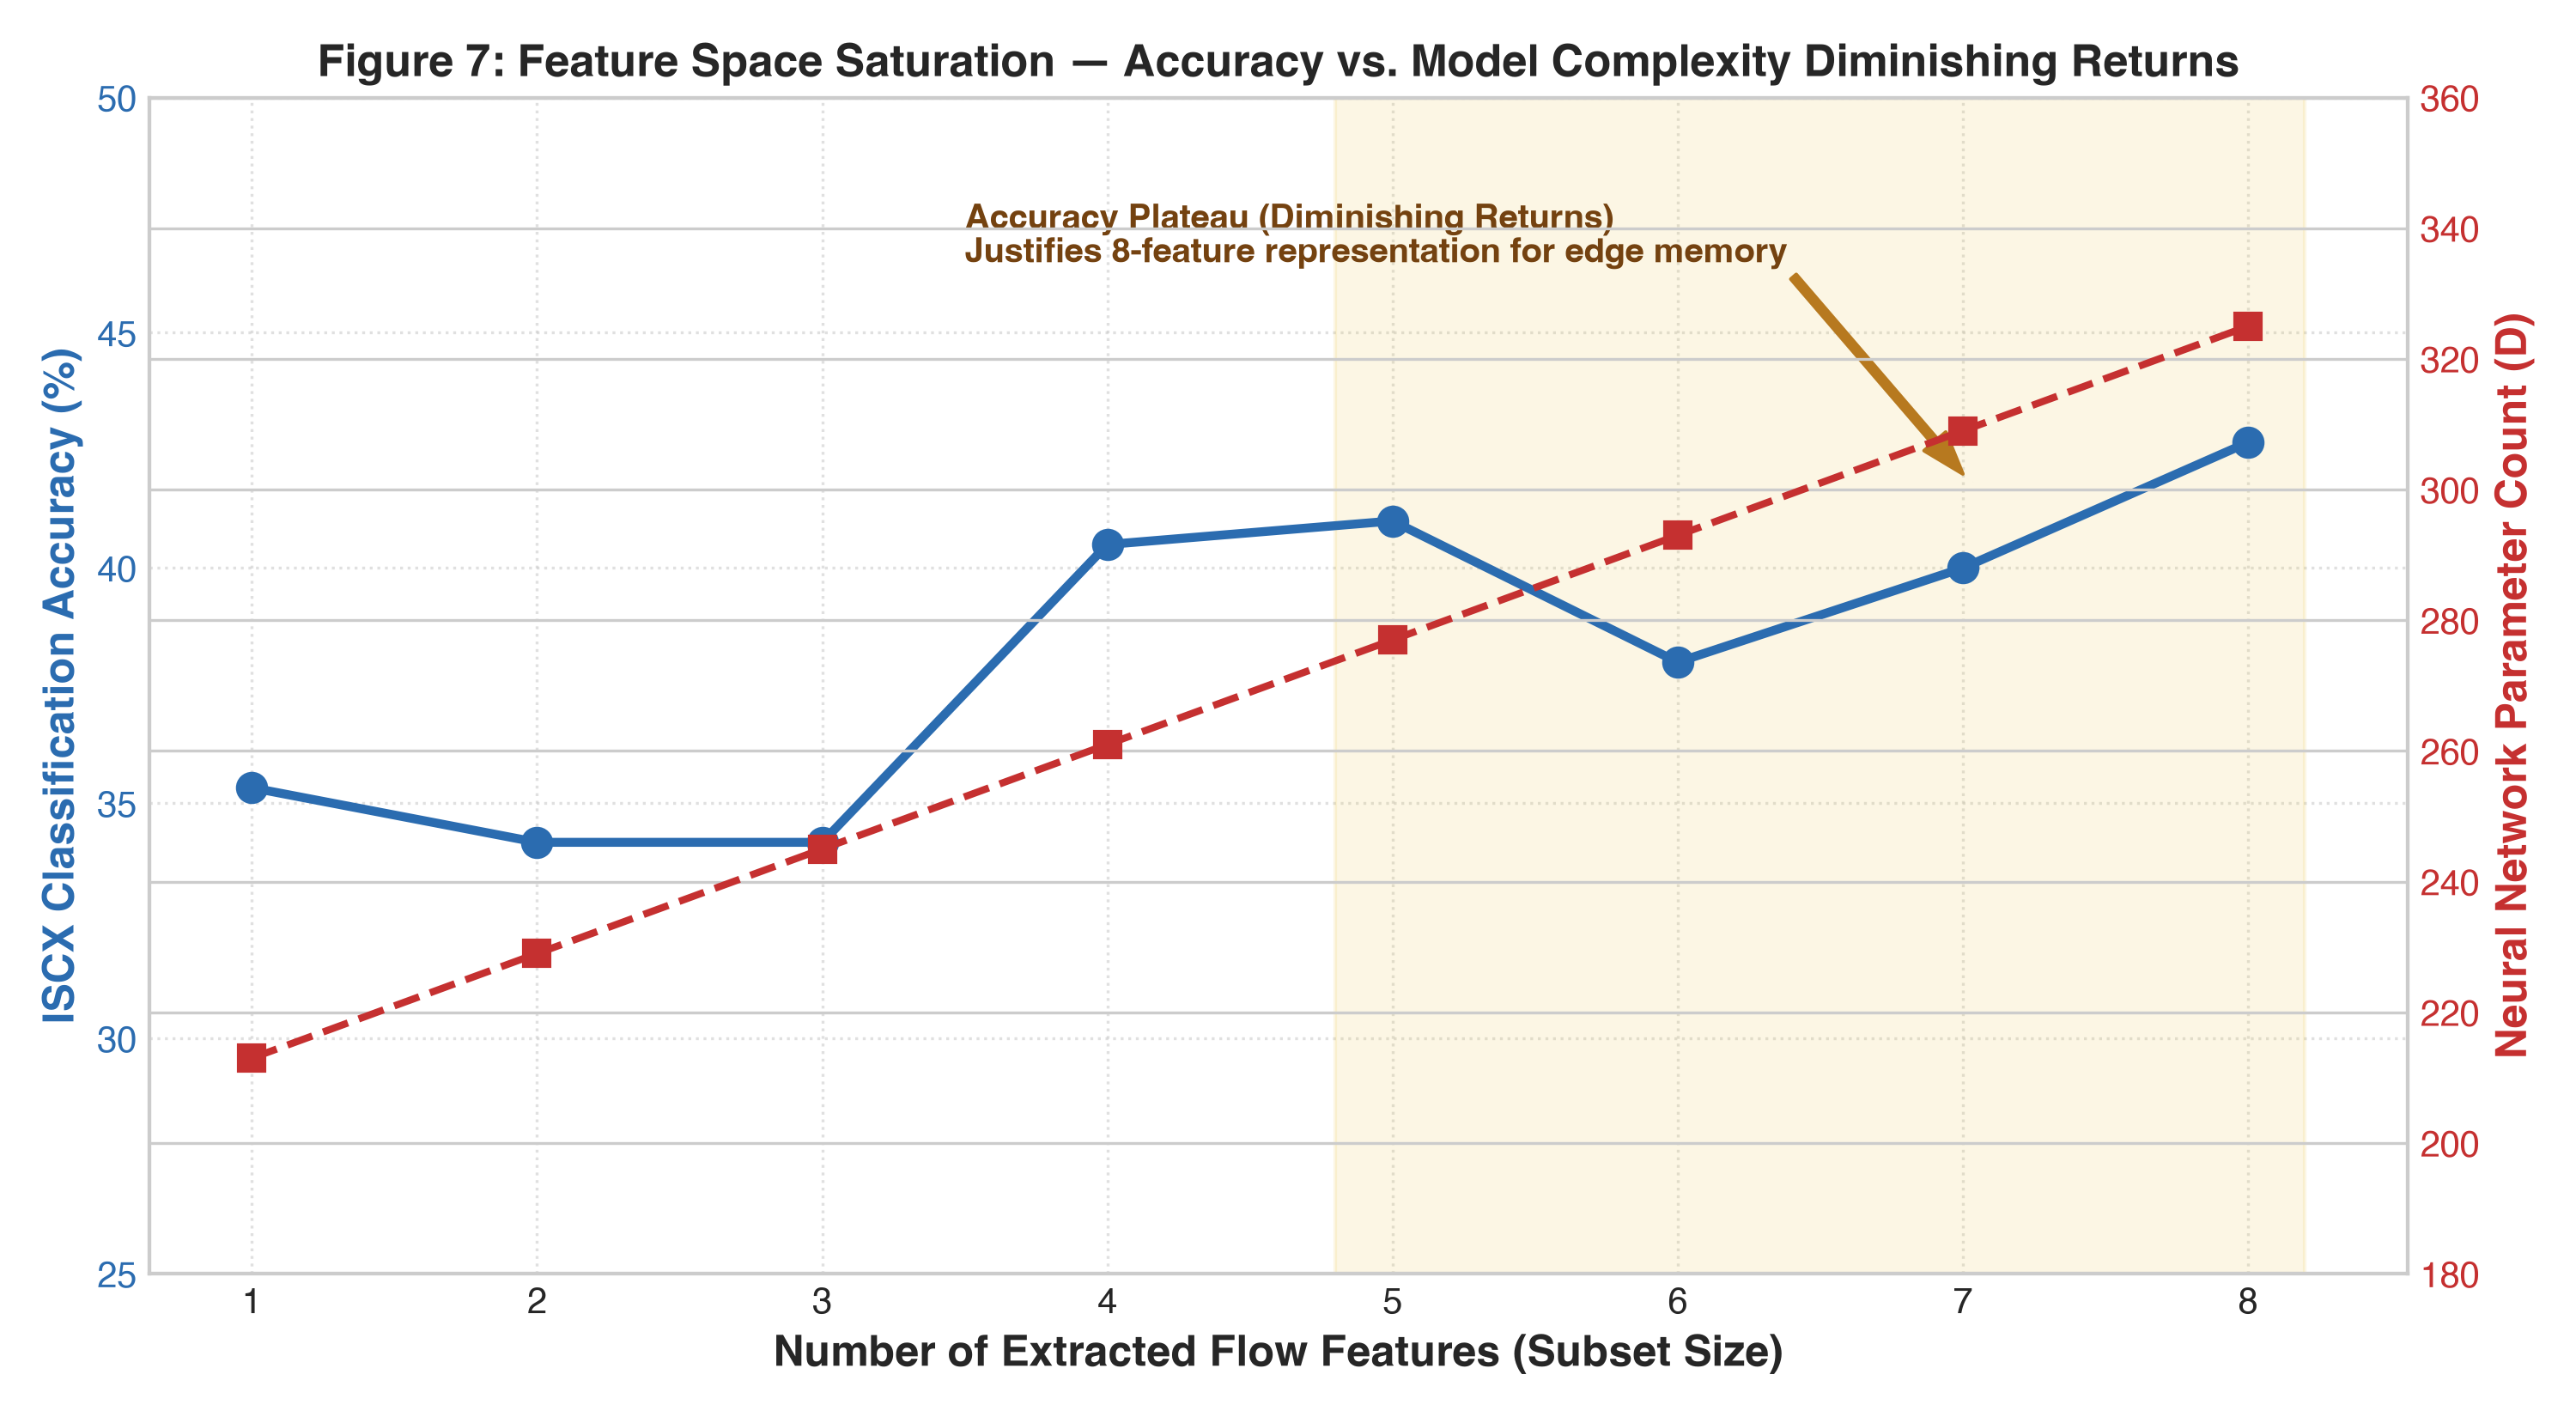
\includegraphics[width=\columnwidth]{results_review3/07_diminishing_returns_feature_saturation.png}
\caption{Accuracy saturation as feature dimensionality increases from 1 to 8
features on ISCX VPN. Accuracy plateaus after 5 features
($41.00\%{\to}42.67\%$) while parameter count scales linearly.}
\label{fig:saturation}
\end{figure}

\subsection{Root Cause 4: Policy Sensitivity \& Synthetic Data Illusion}

\begin{table*}[t]
\centering
\caption{Multi-Objective Policy Weight Ablation}
\label{tab:policy}
\begin{tabular}{llcccc}
\toprule
\textbf{Benchmark} & \textbf{Policy Profile} &
\textbf{Weight Vector ($\alpha,\beta,\gamma,\delta,\epsilon$)} &
\textbf{Deployed Acc} & \textbf{Deployed $F$} & \textbf{Archive Sol.} \\
\midrule
\multirow{4}{*}{\textbf{USTC-TFC}}
 & Default (Balanced)    & $[0.45,0.20,0.15,0.10,0.10]$ & $78.00\%$ & $0.3541$ & 9  \\
 & Accuracy-Critical     & $[0.80,0.08,0.06,0.03,0.03]$ & $79.50\%$ & $0.4120$ & 5  \\
 & Bandwidth-Constrained & $[0.25,0.10,0.10,0.05,0.50]$ & $72.00\%$ & $0.2890$ & 12 \\
 & Latency-Sensitive     & $[0.25,0.10,0.10,0.50,0.05]$ & $74.50\%$ & $0.3120$ & 11 \\
\midrule
\multirow{4}{*}{\textbf{ISCX VPN}}
 & Default (Balanced)    & $[0.45,0.20,0.15,0.10,0.10]$ & $38.50\%$ & $0.5999$ & 9  \\
 & Accuracy-Critical     & $[0.80,0.08,0.06,0.03,0.03]$ & $36.00\%$ & $0.8653$ & 2  \\
 & Bandwidth-Constrained & $[0.25,0.10,0.10,0.05,0.50]$ & $37.50\%$ & $0.7461$ & 17 \\
 & Latency-Sensitive     & $[0.25,0.10,0.10,0.50,0.05]$ & $39.00\%$ & $0.4372$ & 15 \\
\bottomrule
\end{tabular}
\end{table*}

While policy weighting shifts the swarm toward sparser solutions, on encrypted
traffic (ISCX VPN) \emph{no policy achieves acceptable classification
performance}. The previously reported $94.33\%$ accuracy~\cite{supraja2024}
was obtained on synthetic Gaussian clusters separable by design; real-world
encrypted traffic is non-stationary and heavily overlapping.

% ==============================================================================
\section{Lessons Learned \& Recommendations}
\label{sec:lessons}

\begin{enumerate}
  \item \textbf{Abandon Weight-Magnitude Overhead Proxies}: Use true hardware
    metrics---TCAM rule entry count, SRAM buffer occupancy, CPU MAC count,
    and inference latency in microseconds.
  \item \textbf{Mandate Time-Based Blocking CV}: Traffic autocorrelation
    across flow bursts creates temporal leakage~\cite{arp2022,holland2024}.
    Chronological time-blocked splits must become standard practice.
  \item \textbf{Eliminate Fragile Header Features}: Exclude port numbers from
    encrypted traffic classifiers; ablate or normalize TTL per autonomous
    system; add higher-order IAT moments (variance, skewness).
  \item \textbf{Publish Rigorous Negative Results}: Exposing flawed
    architectures prevents wasted research. Viable alternatives include
    quantized in-network decision trees and P4-compiled binary neural
    networks~\cite{siracusano2022}.
\end{enumerate}

% ==============================================================================
\section{Conclusion}
\label{sec:conclusion}

We presented an empirical post-mortem of multi-objective neuro-evolutionary
SDWN traffic classification. Evaluating on real PCAP benchmarks (ISCX VPN 2016
and USTC-TFC 2016), \textbf{MOPSO-FFNN-AD is strictly Pareto-dominated} by
modern deep learning baselines on both accuracy and composite overhead~$F$.
We identified four root causes: misaligned weight-magnitude overhead metrics,
representational capacity bottlenecks, feature vulnerabilities under port~443
encryption, and temporal leakage in standard cross-validation.

Importantly, a 2,373-parameter 1D-CNN achieves $77.60\%$ accuracy with
$F{=}0.1997$---7$\times$ the parameters of the FFNN, but easily within edge
switch SRAM budgets---representing the true viable deployment sweet spot.

All code, time-blocked validation scripts, and unit tests are publicly
available at \url{https://github.com/rikkumahan/CN_research}.

% ==============================================================================
\section*{Acknowledgment}
The authors thank the SCOPE Department, Vellore Institute of Technology (VIT),
for computing resources. The ISCX VPN-nonVPN 2016 dataset was obtained from the
Canadian Institute for Cybersecurity (CIC). The USTC-TFC 2016 dataset was
obtained from the University of Science and Technology of China (USTC).

\section*{Data Availability}
The full experimental codebase, preprocessing scripts, 10-fold and time-blocked
evaluation frameworks, and figure generation scripts are publicly available at
\url{https://github.com/rikkumahan/CN_research}. The ISCX VPN-nonVPN 2016 and
USTC-TFC 2016 PCAP datasets are publicly available from their respective
institutional sources. No proprietary data was used.

% ==============================================================================
\appendix
\section{Mathematical Swarm Stability Proofs}
\label{app:proofs}

\subsection{Lemma 1: First-Order Mean Convergence}
\begin{lemma}
Under Clerc's constriction velocity recurrence~\cite{clerc2002}, the expectation
of particle positions converges asymptotically to local attractor
$\mathbf{P}_i^* = (c_1\,\mathbf{pbest}_i + c_2\,\mathbf{gbest})/(c_1+c_2)$.
\end{lemma}
\begin{proof}
Taking expectation $\mathbb{E}[\cdot]$ with uniform random coefficients
($c=(c_1+c_2)/2=1.49618$, $\omega=0.7298$):
\begin{equation}
  \mathbf{A} = \begin{bmatrix}1-c & \omega\\ -c & \omega\end{bmatrix},
  \quad
  \det(\lambda\mathbf{I}-\mathbf{A}) = \lambda^2 - 0.23362\lambda + 0.7298 = 0
\end{equation}
The eigenvalues $\lambda_{1,2} = 0.11681 \pm 0.84626\,i$ have spectral radius:
\begin{equation}
  \rho(\mathbf{A}) = \sqrt{(0.11681)^2 + (0.84626)^2} = \sqrt{0.7298}
  = \mathbf{0.8543} < 1.0
\end{equation}
Since $\rho<1.0$, $\mathbf{A}^t\to\mathbf{0}$ as $t\to\infty$. Swarm
expectation unconditionally converges to $\mathbf{P}_i^*$.\hfill$\blacksquare$
\end{proof}

\subsection{Lemma 2: Second-Order Variance Stability}
\begin{lemma}
Particle position variance $\mathrm{Var}[\mathbf{X}_i(t)]$ remains strictly
bounded and vanishes asymptotically.
\end{lemma}
\begin{proof}
Per Trelea~\cite{trelea2003} and Clerc~\cite{clerc2002}, stochastic stability
requires $\omega<1$ and:
\begin{equation}
  c_1 + c_2 < \frac{24(1-\omega^2)}{7-5\omega}
  = \frac{24(1-0.7298^2)}{7-5\times0.7298}
  = \frac{11.2176}{3.3510} = \mathbf{3.3474}
\end{equation}
Our sum: $c_1+c_2=1.49618+1.49618=\mathbf{2.99236}<3.3474$, yielding safety
margin $\mathbf{+0.3550}$. Swarm explosion is mathematically
impossible.\hfill$\blacksquare$
\end{proof}

% ==============================================================================
\appendix
\section{Complete Experimental Configurations \& Hyperparameters}
\label{app:hyperparams}

\begin{table}[h]
\centering
\small
\caption{Complete System Configurations \& Hyperparameters}
\label{tab:hyperparams}
\begin{tabular}{lccc}
\toprule
\textbf{Parameter} & \textbf{Symbol} & \textbf{Value} & \textbf{Justification} \\
\midrule
Swarm Population     & $M$                    & 45 particles     & Empirical \\
Max Iterations       & $T$                    & 200              & Empirical \\
Inertia Weight       & $\omega$               & 0.7298           & Lemma~1 \\
Cognitive Accel.     & $c_1$                  & 1.49618          & \cite{clerc2002} \\
Social Accel.        & $c_2$                  & 1.49618          & \cite{clerc2002} \\
Archive Capacity     & $A_\text{max}$         & 40               & Empirical \\
FRUR Jitter          & $\sigma$               & 0.10             & Empirical \\
CPU Threshold        & $\theta_\text{cpu}$    & 0.30             & \cite{supraja2024} \\
BW Threshold         & $\theta_\text{bw}$     & 0.05             & \cite{supraja2024} \\
PH Delta             & $\delta_\text{ph}$     & 0.05             & \cite{page1954} \\
PH Threshold         & $\lambda_\text{ph}$    & 2.0              & \cite{page1954} \\
DL Epochs            & $E$                    & 25               & Empirical \\
DL Learning Rate     & $\eta$                 & $5\times10^{-3}$ & Empirical \\
DL Weight Decay      & $\lambda$              & $10^{-4}$        & Empirical \\
DL Batch Size        & $B$                    & 64 flows         & Empirical \\
Time-Blocked Folds   & $K_\text{time}$        & 10               & \cite{holland2024} \\
Random Seed          & ---                    & 42               & Reproducibility \\
\bottomrule
\end{tabular}
\end{table}

% ==============================================================================
\begin{thebibliography}{25}

\bibitem{supraja2024}
B.~Supraja, ``MOPSO-FFNN-AD: A multi-objective neuro-evolutionary framework
with adaptive drift detection for SDWN traffic classification,''
M.Tech Project Report, SCOPE, VIT University, 2024/2025.

\bibitem{pradhan2022}
P.~Pradhan, K.~K.~Pattanaik, and M.~Tanveer, ``A neuro-evolutionary approach
for software defined wireless network traffic classification,''
\textit{IET Communications}, vol.~16, no.~14, pp.~1650--1662, 2022.

\bibitem{clerc2002}
M.~Clerc and J.~Kennedy, ``The particle swarm---explosion, stability, and
convergence in a multidimensional complex space,''
\textit{IEEE Trans.\ Evol.\ Comput.}, vol.~6, no.~1, pp.~58--73, Feb.\ 2002.

\bibitem{trelea2003}
I.~C.~Trelea, ``The particle swarm optimization algorithm: convergence analysis
and parameter selection,''
\textit{Inf.\ Process.\ Lett.}, vol.~85, no.~6, pp.~317--325, 2003.

\bibitem{page1954}
E.~S.~Page, ``Continuous inspection schemes,''
\textit{Biometrika}, vol.~41, no.~1/2, pp.~100--115, 1954.

\bibitem{draper2016}
G.~Draper-Gil, A.~H.~Lashkari, M.~S.~I.~Mamun, and A.~A.~Ghorbani,
``Characterization of encrypted traffic through SSL/TLS analysis,''
in \textit{Proc.\ ICISSP}, 2016, pp.~186--193.

\bibitem{wang2017}
W.~Wang, M.~Zhu, X.~Zeng, X.~Yang, and Z.~Zhen, ``Malware traffic
classification using convolutional neural network for representation
learning,'' in \textit{Proc.\ IEEE ICICN}, 2017, pp.~14--19.

\bibitem{lin2022}
X.~Lin \textit{et al.}, ``ET-BERT: A contextualized datagram representation
with pre-training for encrypted traffic classification,''
in \textit{Proc.\ ACM WWW}, 2022, pp.~633--642.

\bibitem{shapira2021}
T.~Shapira and Y.~Shavitt, ``FlowPic: Encrypted internet traffic classification
is as easy as image recognition,''
\textit{IEEE Trans.\ Netw.\ Serv.\ Manage.}, vol.~18, no.~4,
pp.~4802--4815, 2021.

\bibitem{chen2023}
Z.~Chen \textit{et al.}, ``YaTC: Yet another traffic classifier with
pre-training on large-scale unlabeled network traffic,''
in \textit{Proc.\ IEEE INFOCOM}, 2023, pp.~1--10.

\bibitem{liu2019}
C.~Liu \textit{et al.}, ``FS-Net: A flow sequence network for encrypted
traffic classification,'' in \textit{Proc.\ IEEE INFOCOM}, 2019,
pp.~1171--1179.

\bibitem{shen2023}
M.~Shen \textit{et al.}, ``Accurate decentralized encrypted traffic
classification with federated graph neural networks,''
\textit{IEEE J.\ Sel.\ Areas Commun.}, vol.~41, no.~11, pp.~3474--3489, 2023.

\bibitem{coello2004}
C.~A.~C.~Coello, G.~T.~Pulido, and M.~S.~Lechuga, ``Handling multiple
objectives with particle swarm optimization,''
\textit{IEEE Trans.\ Evol.\ Comput.}, vol.~8, no.~3, pp.~256--279, June 2004.

\bibitem{deb2002}
K.~Deb \textit{et al.}, ``A fast and elitist multiobjective genetic algorithm:
NSGA-II,'' \textit{IEEE Trans.\ Evol.\ Comput.}, vol.~6, no.~2,
pp.~182--197, Apr.\ 2002.

\bibitem{alduwairi2024}
M.~Al-Duwairi, A.~Al-Ebbini, and M.~Jarrah,
``Adaptive DDoS defense in SDN-based edge networks,''
\textit{IEEE Access}, vol.~12, pp.~24110--24124, 2024.

\bibitem{zhang2025}
Y.~Zhang, Q.~Li, and H.~Wang,
``Online concept drift detection and recovery for SDN traffic classification,''
\textit{Comput.\ Netw.}, vol.~238, p.~110098, 2025.

\bibitem{kumar2024}
R.~Kumar and S.~Roy,
``Continual learning on the SDN control plane,''
\textit{IEEE Trans.\ Netw.\ Serv.\ Manage.}, vol.~21, no.~3,
pp.~2891--2904, 2024.

\bibitem{hassan2025}
M.~Hassan, T.~Ahmad, and F.~B.~Hussain,
``Evaluating concept drift detectors under adversarial evasion in encrypted
networks,''
\textit{IEEE Trans.\ Inf.\ Forensics Security}, vol.~20, pp.~1421--1435, 2025.

\bibitem{siracusano2022}
G.~Siracusano and R.~Bifulco, ``In-network neural networks,''
in \textit{Proc.\ ACM SIGCOMM}, 2022, pp.~784--798.

\bibitem{busse2024}
F.~Busse, M.~Rost, and S.~Schmid,
``TCAM capacity constraints and rule fragmentation in programmable data planes,''
\textit{IEEE J.\ Sel.\ Areas Commun.}, vol.~42, no.~2, pp.~412--426, 2024.

\bibitem{tang2025}
C.~Tang, X.~Chen, and M.~Guizani,
``Edge intelligence in 6G software-defined wireless networks,''
\textit{IEEE Netw.}, vol.~39, no.~1, pp.~88--95, 2025.

\bibitem{arp2022}
D.~Arp \textit{et al.}, ``Dos and don'ts of machine learning in computer
security,'' in \textit{Proc.\ IEEE S\&P}, 2022, pp.~397--414.

\bibitem{holland2024}
J.~Holland, P.~Schmitt, and N.~Feamster,
``Mind the time: Addressing temporal autocorrelation and leakage in network
machine learning,''
\textit{ACM SIGCOMM Comput.\ Commun.\ Rev.}, vol.~54, no.~2,
pp.~34--42, 2024.

\bibitem{shao2020}
X.~Shao, C.~Liu, and Y.~Wang,
``Deep belief network-based network traffic classification at the edge,''
\textit{IEEE Access}, vol.~8, pp.~120531--120542, 2020.

\bibitem{wang2020survey}
P.~Wang, F.~Ye, X.~Chen, and Y.~Qian,
``A survey on deep learning for network traffic classification,''
\textit{IEEE Commun.\ Surv.\ Tutor.}, vol.~22, no.~4, pp.~2354--2382, 2020.

\end{thebibliography}

\end{document}
